%%
%% licence       kaneton licence
%%
%% project       kaneton
%%
%% file          /home/buckman/kaneton/view/lectures/kernels/tp-k0/tp-k0.tex
%%
%% created       matthieu bucchianeri   [wed jan 24 14:46:51 2007]
%% updated       matthieu bucchianeri   [thu jan 25 00:11:03 2007]
%%

%
% template
%

%
% ---------- header -----------------------------------------------------------
%
% project       kaneton
%
% license       kaneton
%
% file          /home/mycure/kaneton/view/template/paper.tex
%
% created       julien quintard   [wed may 16 18:17:37 2007]
% updated       julien quintard   [fri oct  5 07:00:45 2007]
%

%
% class
%

\documentclass[10pt,a4wide]{article}

%
% packages
%

\usepackage[english]{babel}
\usepackage[T1]{fontenc}
\usepackage{a4wide}
\usepackage{fancyheadings}
\usepackage{multicol}
\usepackage{indentfirst}
\usepackage{graphicx}
\usepackage{color}
\usepackage{xcolor}
\usepackage{verbatim}
\usepackage{aeguill}

\pagestyle{fancy}

\setlength{\footrulewidth}{0.3pt}
\setlength{\parindent}{0.3cm}
\setlength{\parskip}{2ex plus 0.5ex minus 0.2ex}

%
% logos
%

\newcommand{\logos}
  {
    \begin{center}
      
\includegraphics[scale=0.8]{\path/logo/kaneton.pdf}
    \end{center}
  }

%
% prototype
%

\newcommand\prototype[2]{
  \begin{tabular}{p{0.2cm}p{13.8cm}}
  & #1
  \end{tabular}

  \begin{tabular}{p{1cm}p{13cm}}
  & #2
  \end{tabular}}

%
% verbatim stuff
%

\definecolor{verbatimcolor}{rgb}{0.00,0.40,0.00}

\makeatletter

\renewcommand{\verbatim@font}
  {\ttfamily\footnotesize\selectfont}

\def\verbatim@processline{
  {\color{verbatimcolor}\the\verbatim@line}\par
}

\makeatother

%
% header
%

\rhead{}
\rfoot{\scriptsize{The kaneton microkernel project}}

\date{\scriptsize{\today}}

\usepackage{pdfpages}

%
% header
%

\lhead{\scriptsize{k0}}

%
% title
%

\title{kaneton K0\\Bootstrap}

%
% authors
%

\author{\small{Matthieu Bucchianeri} and
        \small{Renaud Voltz}}

%
% document
%

\begin{document}

\maketitle

\vspace{5mm}

\begin{tabular}{p{7cm}l}
Delivery date: & Sunday, 28th \\
               & 11:42 pm \\
Assistants : & Matthieu Bucchianeri - \small{chichelover@epita.fr} \\
             & Renaud Voltz - \small{voltz\_r@epita.fr} \\
Dedicated googlegroup: & kaneton-students \\
Programming languages: & Assembly, C \\
Architecture: & Intel 32-bit \\
Students per group: & 1
\end{tabular}

\section*{Introduction}

\newpage


\section*{Implementation}

\subsection*{Before starting}

\begin{itemize}
\item
  You will use NASM to assemble your code. NASM is present on the
  PIE. To test, you will use QEMU, which can be ran using the script
  \tt $\tilde{}$bucchi\_m/qemu/run.sh \rm and adding the correct parameters
  (\tt -fda \rm for a floppy image).
\item
  A bootsector is not an ELF binary, but a flat object (without any
  headers). Obtaining flat binaries with NASM is done using the \tt -f \rm
  flag (refer to the manual).
\item
  The bootsector is loaded at address 0x7c00, you must find a way to
  tell NASM that the code will be loaded there.
\item
  Remember that the microprocessor starts in 16-bit mode, so you must
  find a directive to tell NASM to assemble 16-bit code. Next, when
  you switch to 32-bit mode, find another directive to tell NASM the
  new assembly mode.
\end{itemize}

\subsection*{Exercise 1: string display}
Print a string at the (20, 10) coordinates. You must use the BIOS calls.\\
\\
{\bf Steps:}
\begin{enumerate}
\item {\tt print\_char}\\
Print a character at the current cursor position, and update the cursor position.
\item {\tt print\_string}\\
Print the string pointed by {\em \%si} register at the cursor position and update the cursor position.
\item{\tt cursor\_set}\\
Set the cursor position.
\end{enumerate}




\subsection*{Exercise 2: libc}


  \begin{enumerate}
  \item {\tt malloc}\\
  Very stupid malloc:
  \begin{itemize}
  \item Declare the heap.
  \item Declare a break value at the begining of the heap.
  \item malloc returns the break value in {\em \%ax} and then increments it.
  \end{itemize}
  \item {\tt itoa}\\
  Basic itoa (hey, why not using it to test your malloc ?!).
  \item {\tt itoa\_hex}\\
  Hexadecimal itoa (the 0x prefix would be appreciated).
  \item {\tt strcmp}\\
  Basic strcmp : return 0 if both strings are equal, return 1 otherwise.
  \end{enumerate}


\subsection*{Exercise 3: keyboard inputs}

Write a prompt which gets a string from the keyboard and wich displays it when you press {\tt ENTER}.\\
\\
You must display alpha-numeric characters and punctuation.\\
Do not implement key combinations (using modifiers like {\tt SHIFT}, {\tt ALT}, {\tt CTRL}, \ldots).\\
Pressing {\tt ENTER} must result in a newline.\\
\\
{\em Example}:
\begin{verbatim}
Enter your name: Renaud
Hello Renaud !
\end{verbatim}
{\bf Steps:}
  \begin{enumerate}
  \item {\tt kbd\_get\_scancode}\\
  Get the next scancode from the keyboard buffer.
  \item {\tt scancode\_to\_ascii}\\
  Convert a scancode to an ASCII character.
  \end{enumerate}



\subsection*{Exercise 4: floppy drive}

Write a program which loads the bootsector of a floppy disk and which checks wether it does contain a bootloader.\\
\\
(The bootsector contains a bootloader if it is ended by the 0xAA55 magic.)\\
\\
Your program must print the magic value as shown in the following example:\\
\\
{\em Example:}
\begin{verbatim}
Loading floppy bootsector ... OK
magic found: 0xaa55

Loading floppy bootsector ... OK
ERROR: bad magic: 0xt824
\end{verbatim}
{\bf Steps:}
  \begin{enumerate}
  \item {\tt floppy\_read\_sector}\\
  Read {\em n} sectors from the floppy drive (A:).
  \end{enumerate}

\subsection*{Exercise 5: operating modes switching}

Write a program which turns the microprocessor into protected mode.

  \begin{enumerate}
  \item {\tt pmode\_enable}\\
  Switch from real mode to protected mode.
  \item {\tt memset}\\
  Basic memset function.
  \item {\tt memcpy}\\
  Basic memcpy function.
  \end{enumerate}

\subsection*{Exercise 6: ELF loader}

You will now write a complete bootloader. This one will load an ELF
file from the disk (located at the sector just after the bootsector)
and then relocate it in memory at the right place, before jumping to
it.

The ELF file \textbf{must} contains two segments, one with code (which
must be loaded at 1 Mb) and the other with data (loaded at 2
Mb). Example:

\begin{verbatim}
42sh> readelf -l bootloader

Elf file type is EXEC (Executable file)
Entry point 0x1000cc
There are 2 program headers, starting at offset 52

Program Headers:
  Type           Offset   VirtAddr   PhysAddr   FileSiz MemSiz  Flg Align
  LOAD           0x001000 0x00100000 0x00100000 0x000df 0x000df R E 0x1000
  LOAD           0x002000 0x00200000 0x00200000 0x00022 0x00028 RW  0x1000

 Section to Segment mapping:
  Segment Sections...
   00     .text
   01     .data .rodata .bss
\end{verbatim}

Your bootloader \textbf{must} reset the BSS memory. To keep the thing
simple, put the \emph{.bss} section at the end of the second
segment. Its size can be determined by computing the difference
between MemSize and FileSiz.

Your tarball \textbf{must} include the ld-script used to create such
ELF binaries.

Before starting, you should watch the ELF documentation, especially
about the ELF header and the Program Header. The task is not as harder
as it looks like (our code dealing with ELF files is about 30
instructions long).

A good methodology should follow these steps:

  \begin{enumerate}

    \item {Get the \tt floppy\_read\_sector \rm function and call it
    correctly to store the binary in a temporary location}

    \item {Reuse your \tt pmode\_enable \rm function}

    \item {Read the loaded binary to find the segments and extract
    their load addresses, size and source location into the file}

    \item {Use your \tt memcpy \rm to relocate the code and the
    initialized data, use your \tt memset \rm to reset the BSS section}

    \item {Find the binary entry point (2 instructions !) and jump on
    it after initializing a correct stack)}

  \end{enumerate}

You must write your own test ELF binary, which must be able to write
text on the screen. See appendix \emph{VGA text framebuffer}.

\newpage

\section{Appendixes}

\begin{itemize}
\item
  BIOS services:
  \begin{itemize}
  \item
    int 10: video services
  \item
    int 13: disk services
  \item
    int 16: keyboard services
  \end{itemize}
\item
  VGA Text Framebuffer
\item
  Executable \& Linkable Format (ELF) documentation
\item
  Intel IA-32 mode switching procedures
\end{itemize}

%
% Bios interrupts documentation
%

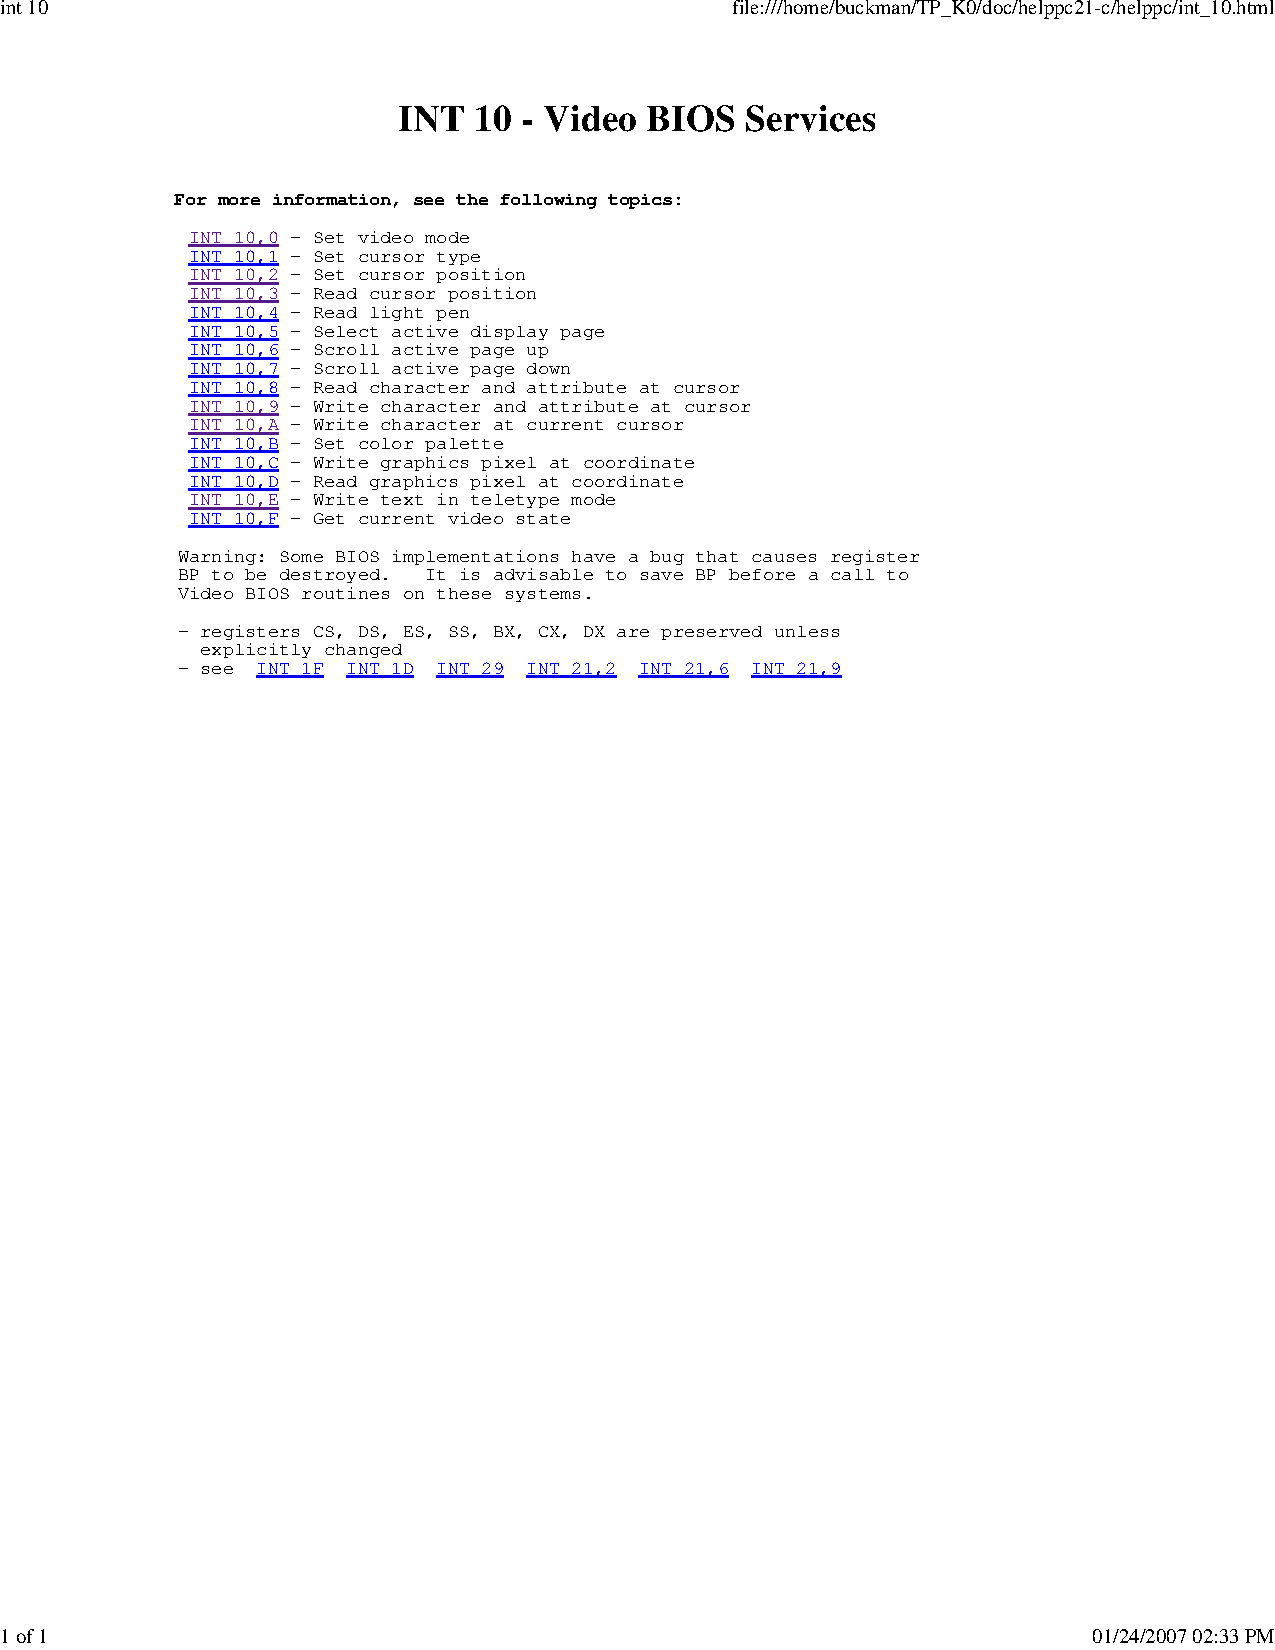
\includepdf[pages=-]{int10}
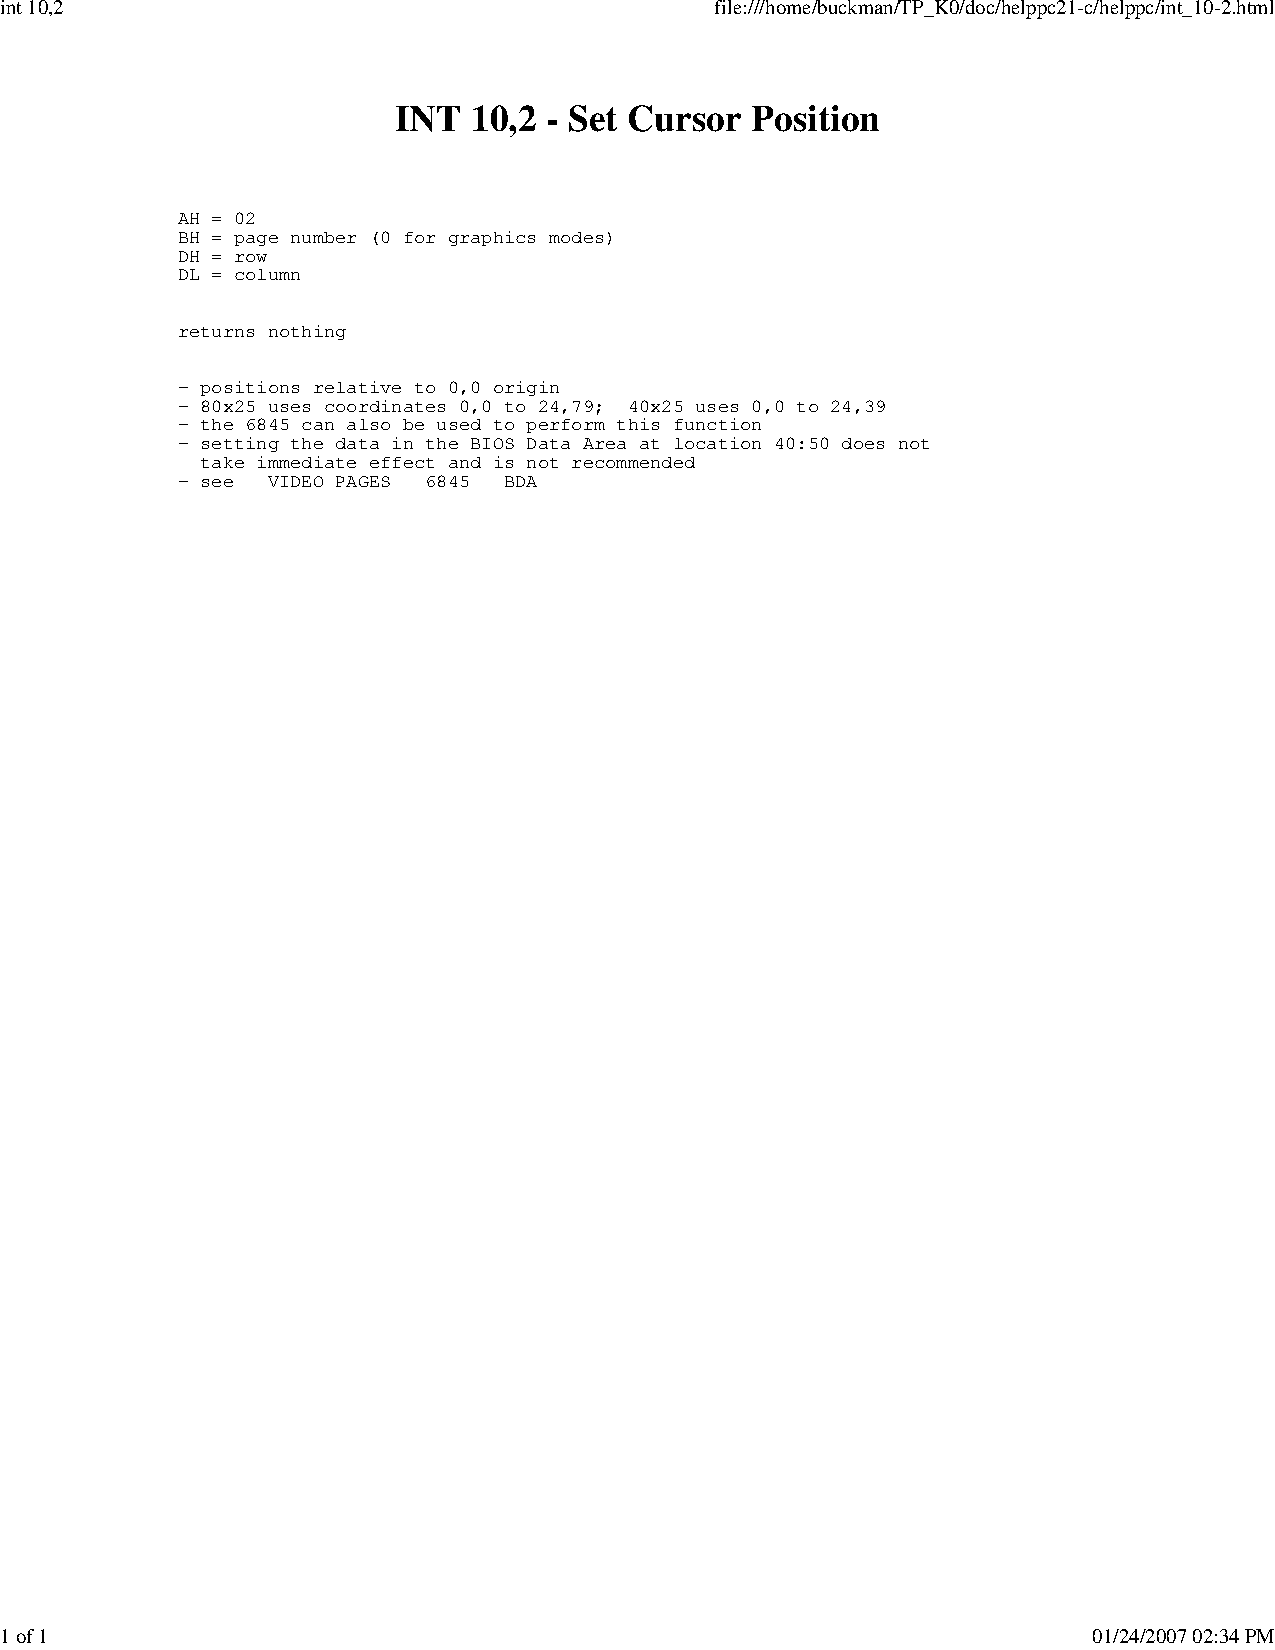
\includepdf[pages=-]{int10_2}
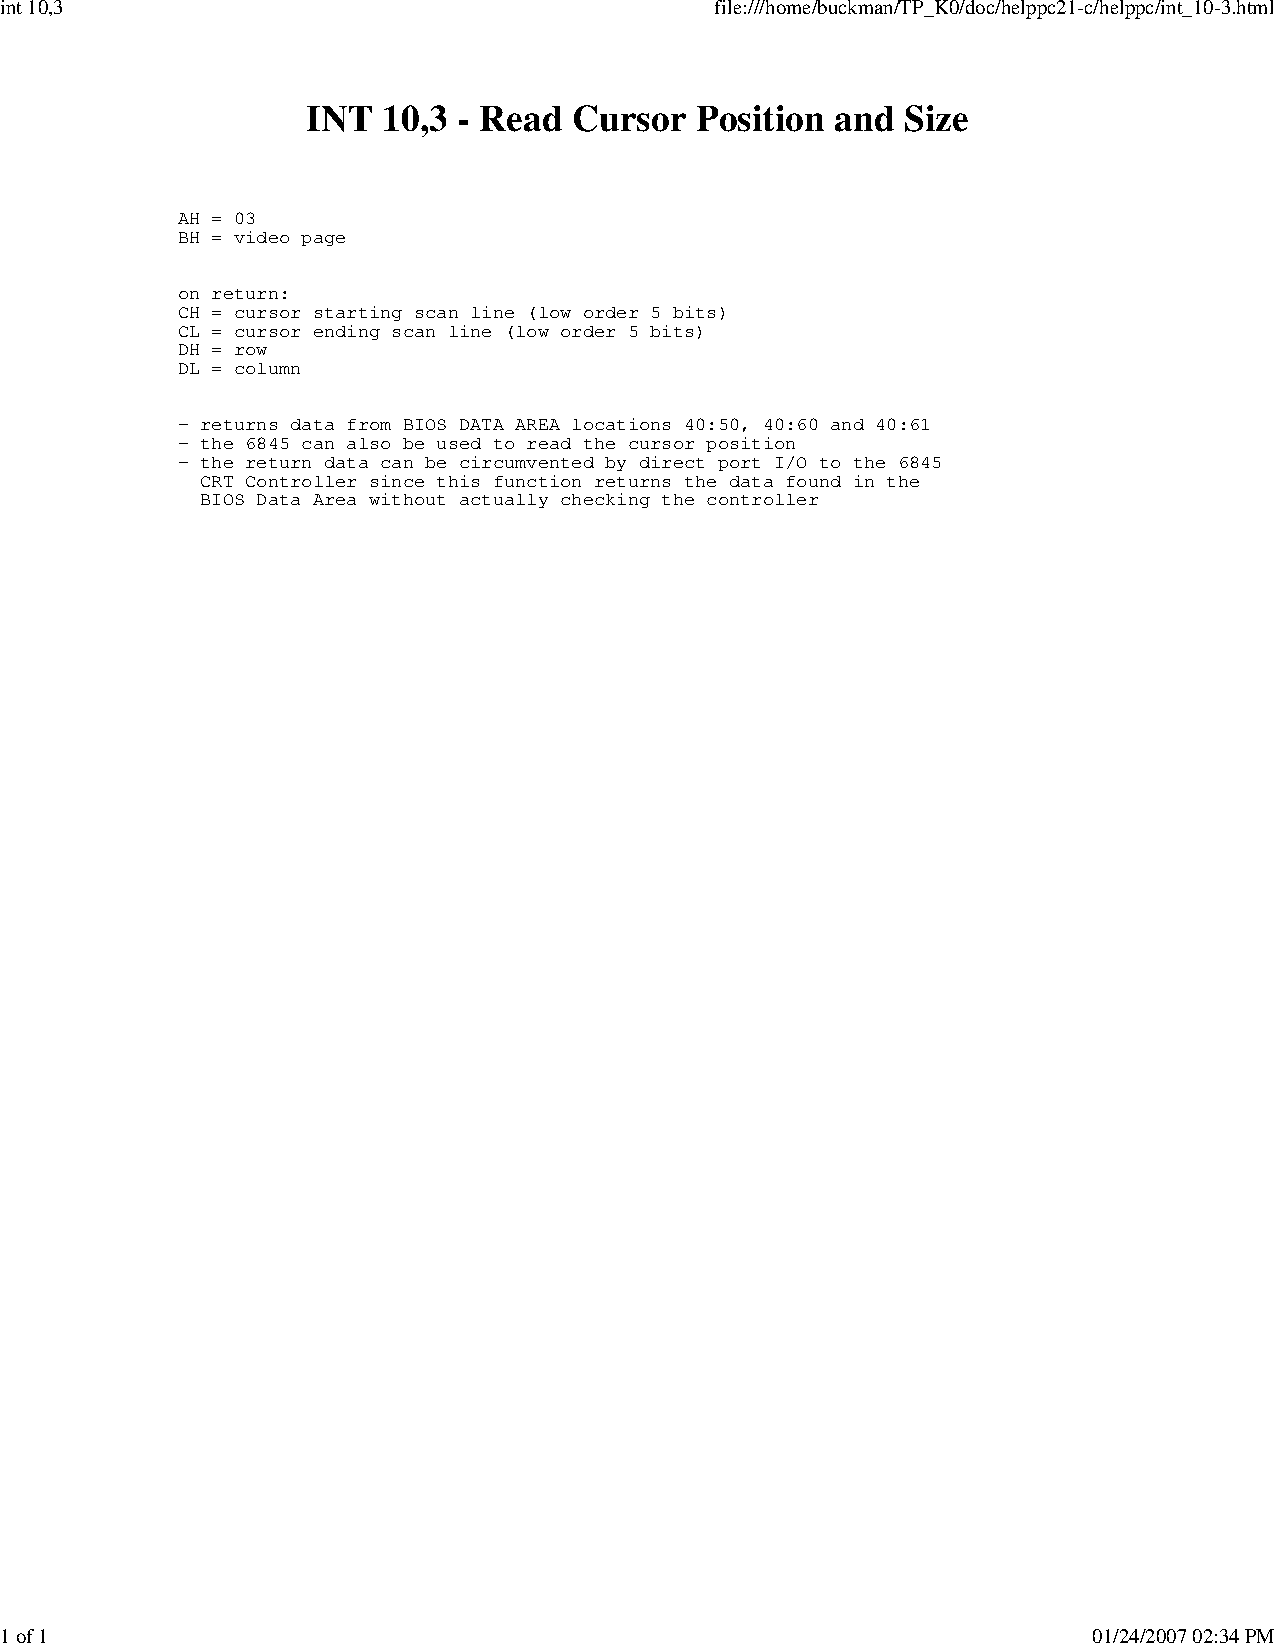
\includepdf[pages=-]{int10_3}
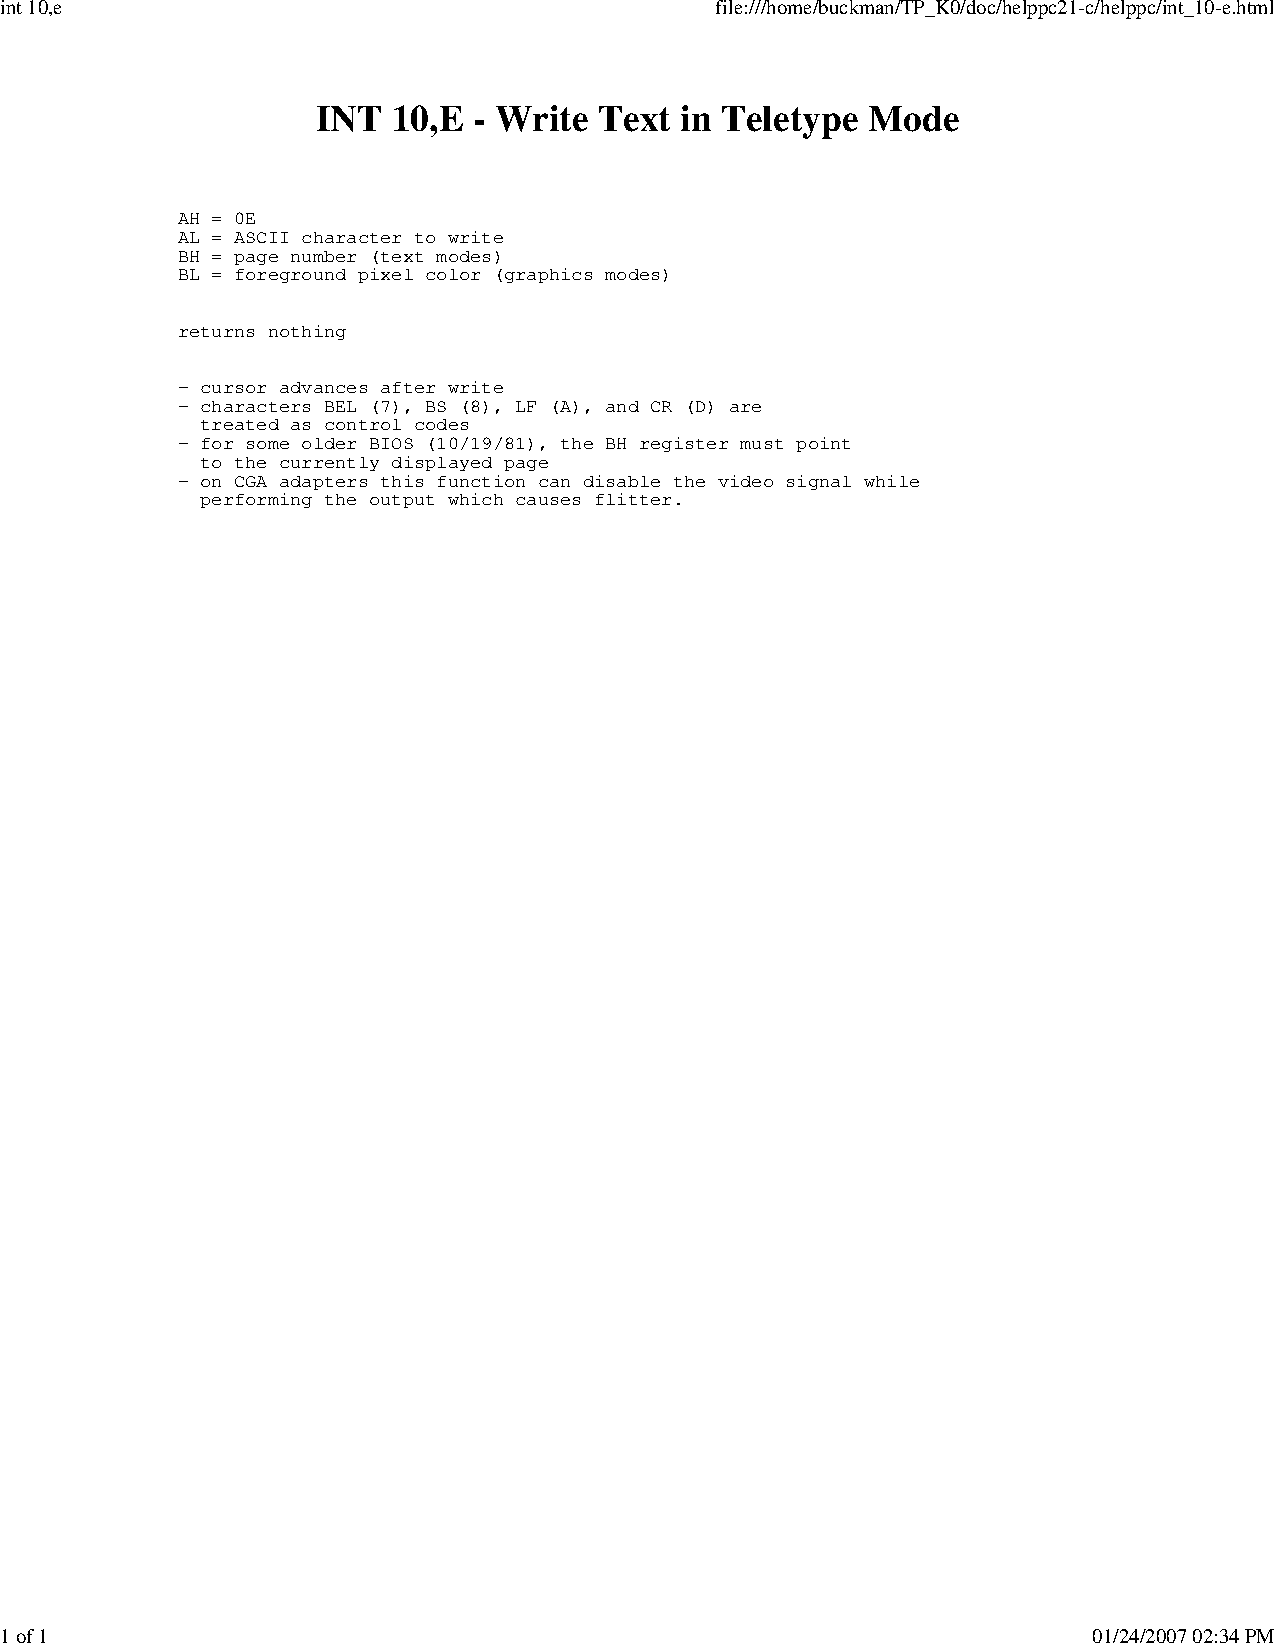
\includepdf[pages=-]{int10_e}

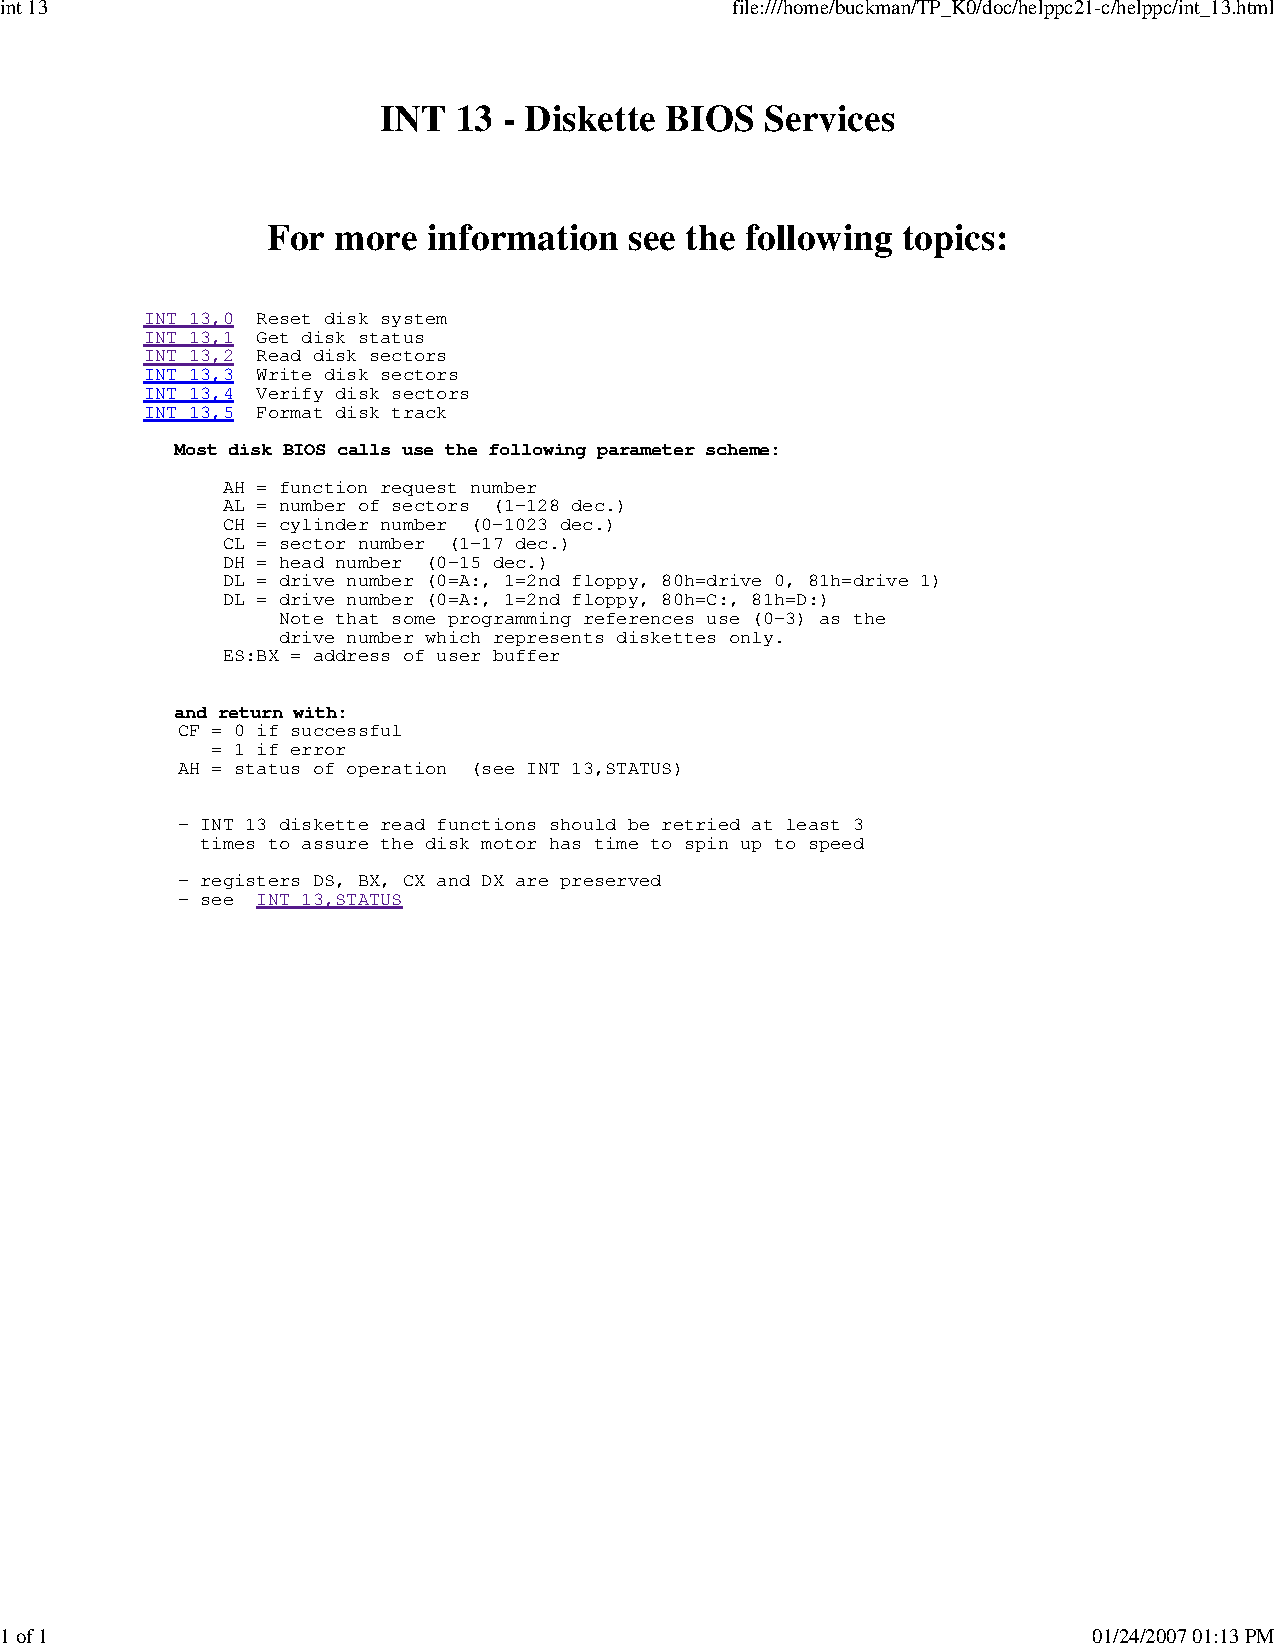
\includepdf[pages=-]{int13}
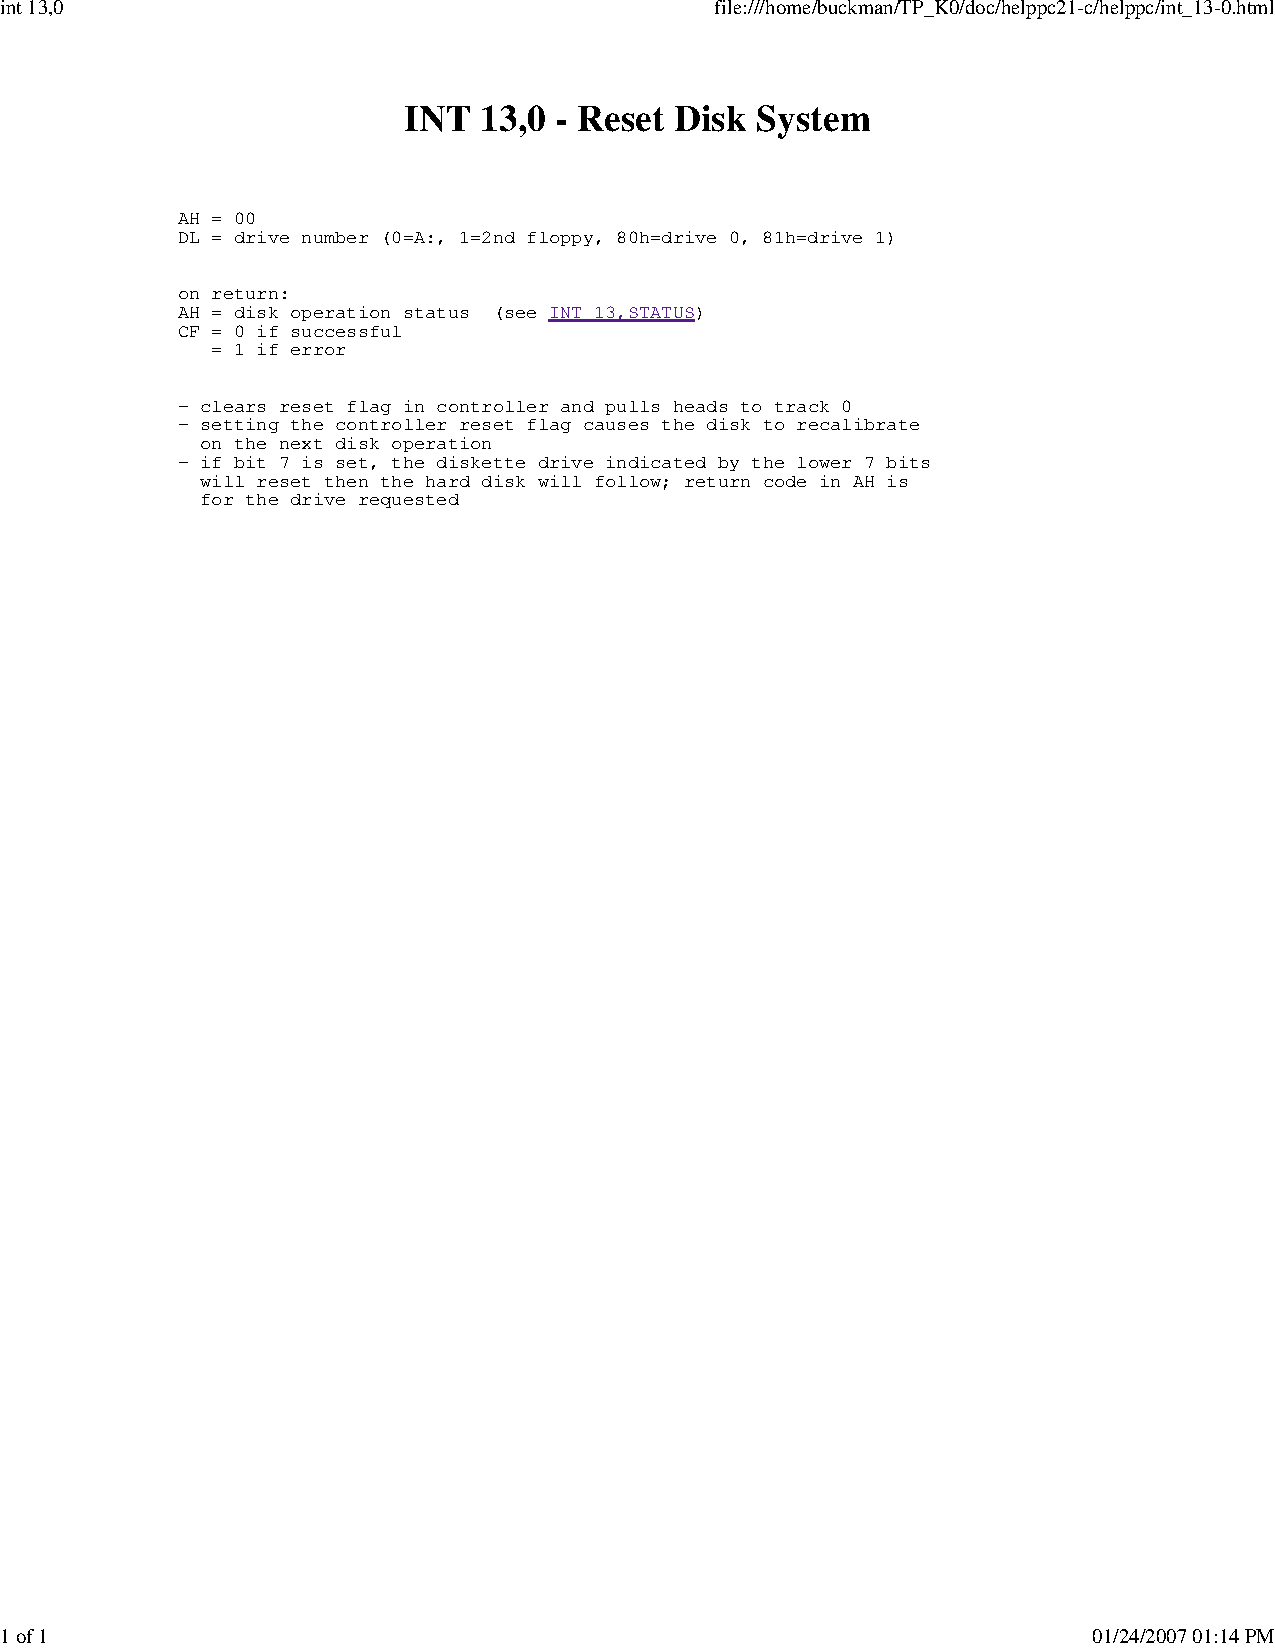
\includepdf[pages=-]{int13_0}
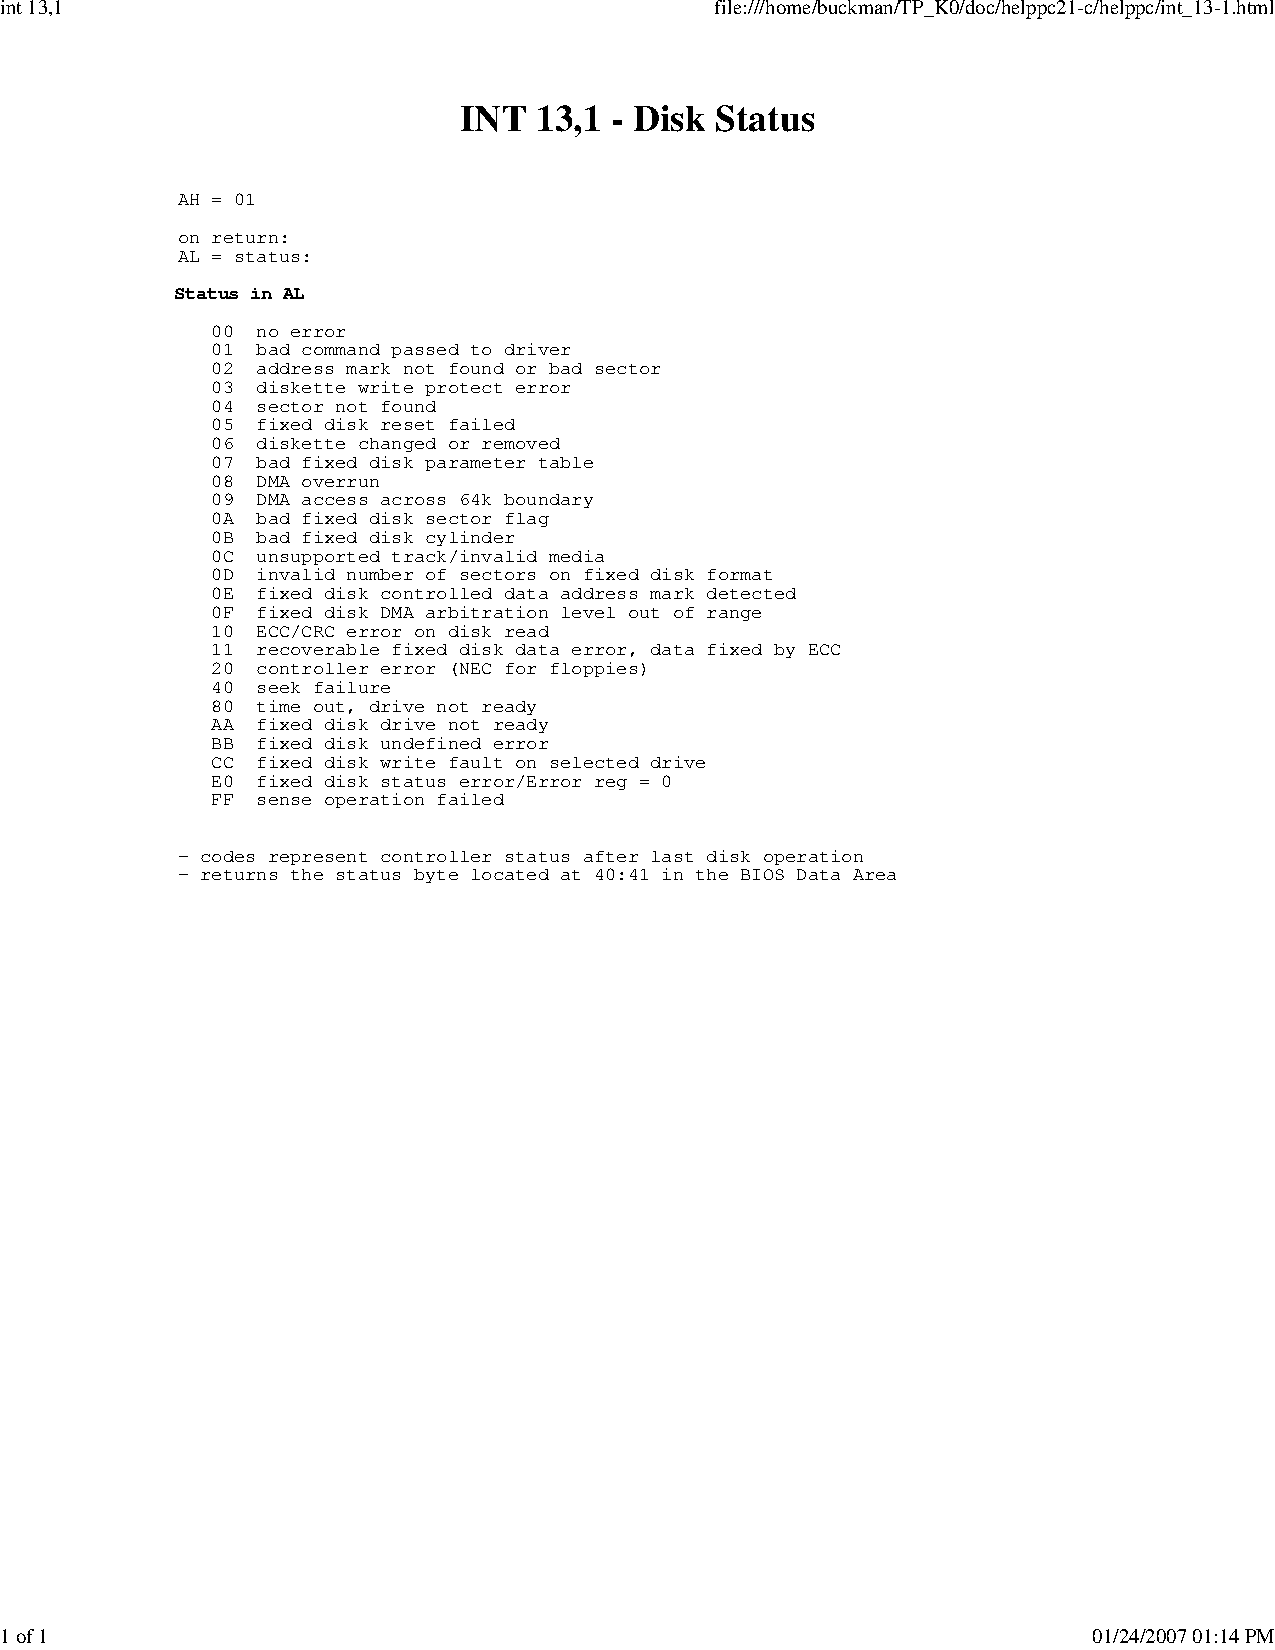
\includepdf[pages=-]{int13_1}
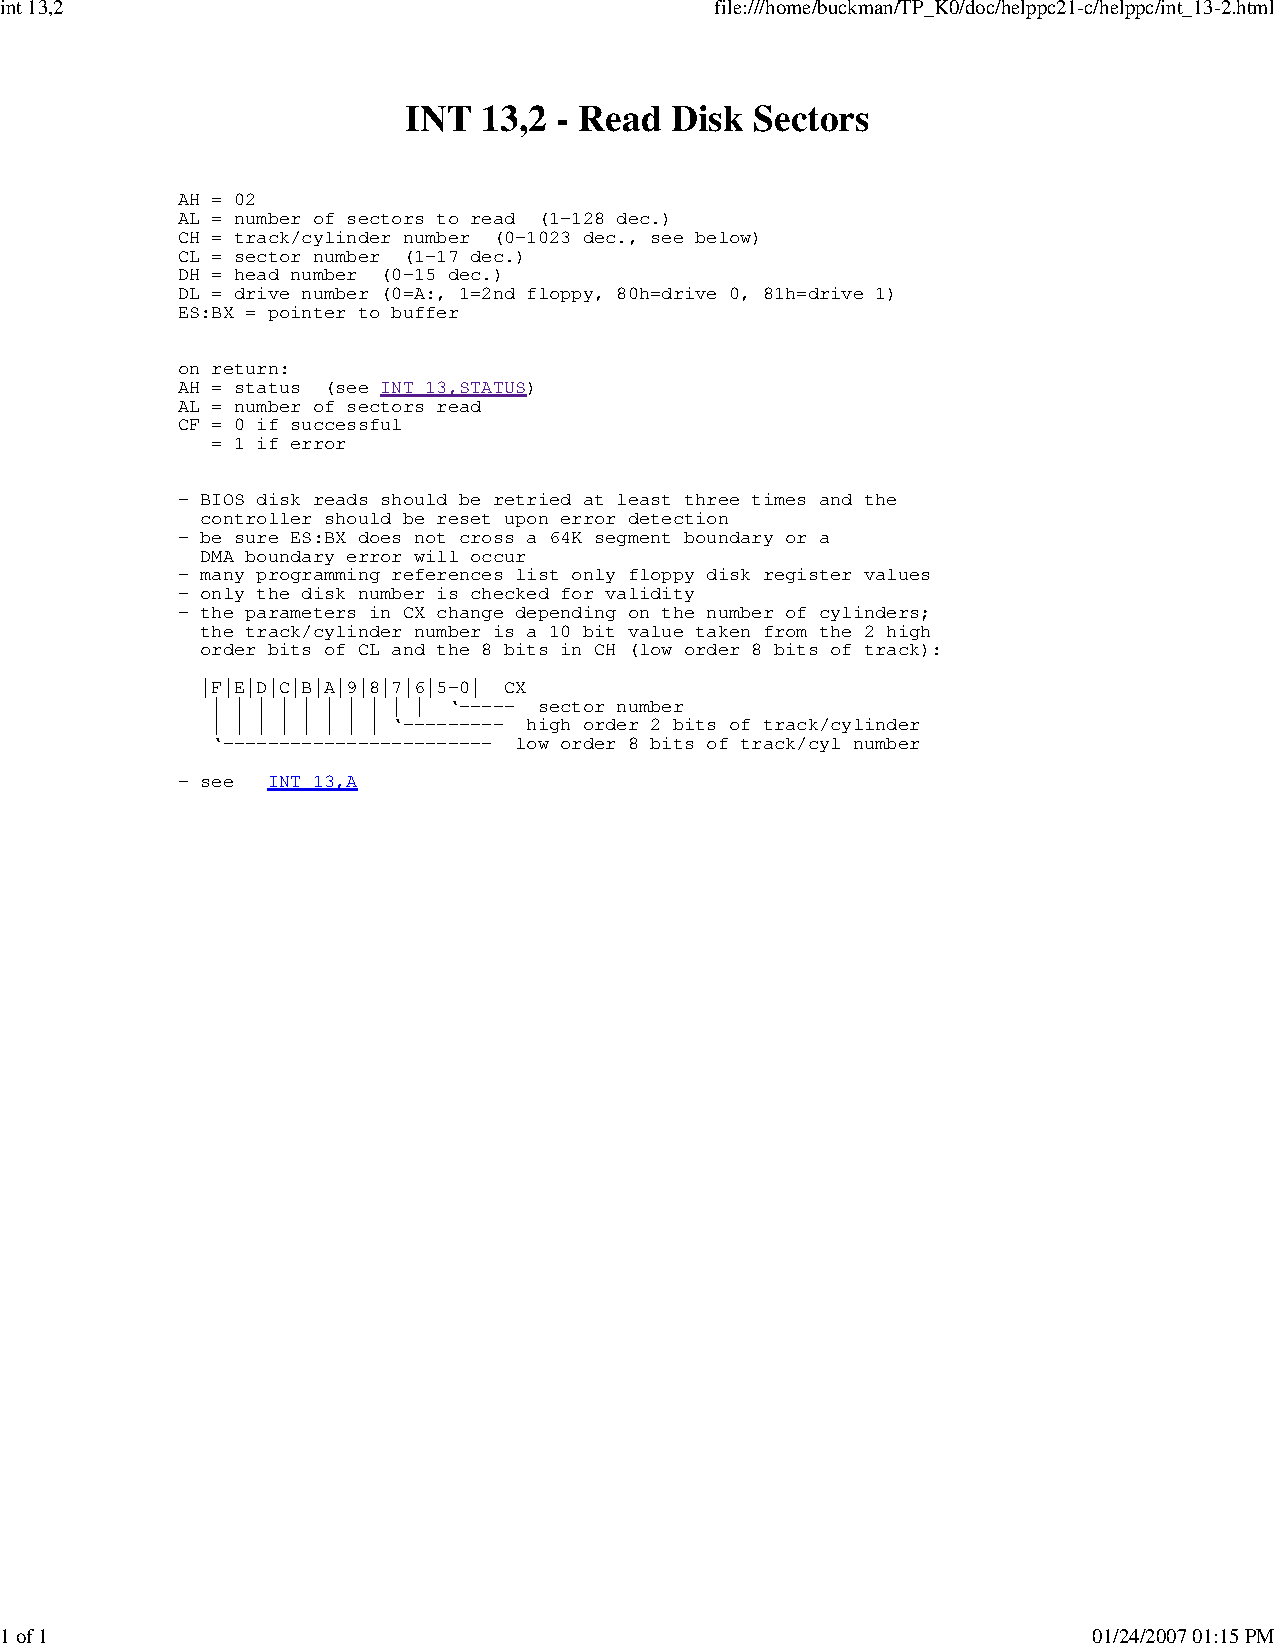
\includepdf[pages=-]{int13_2}

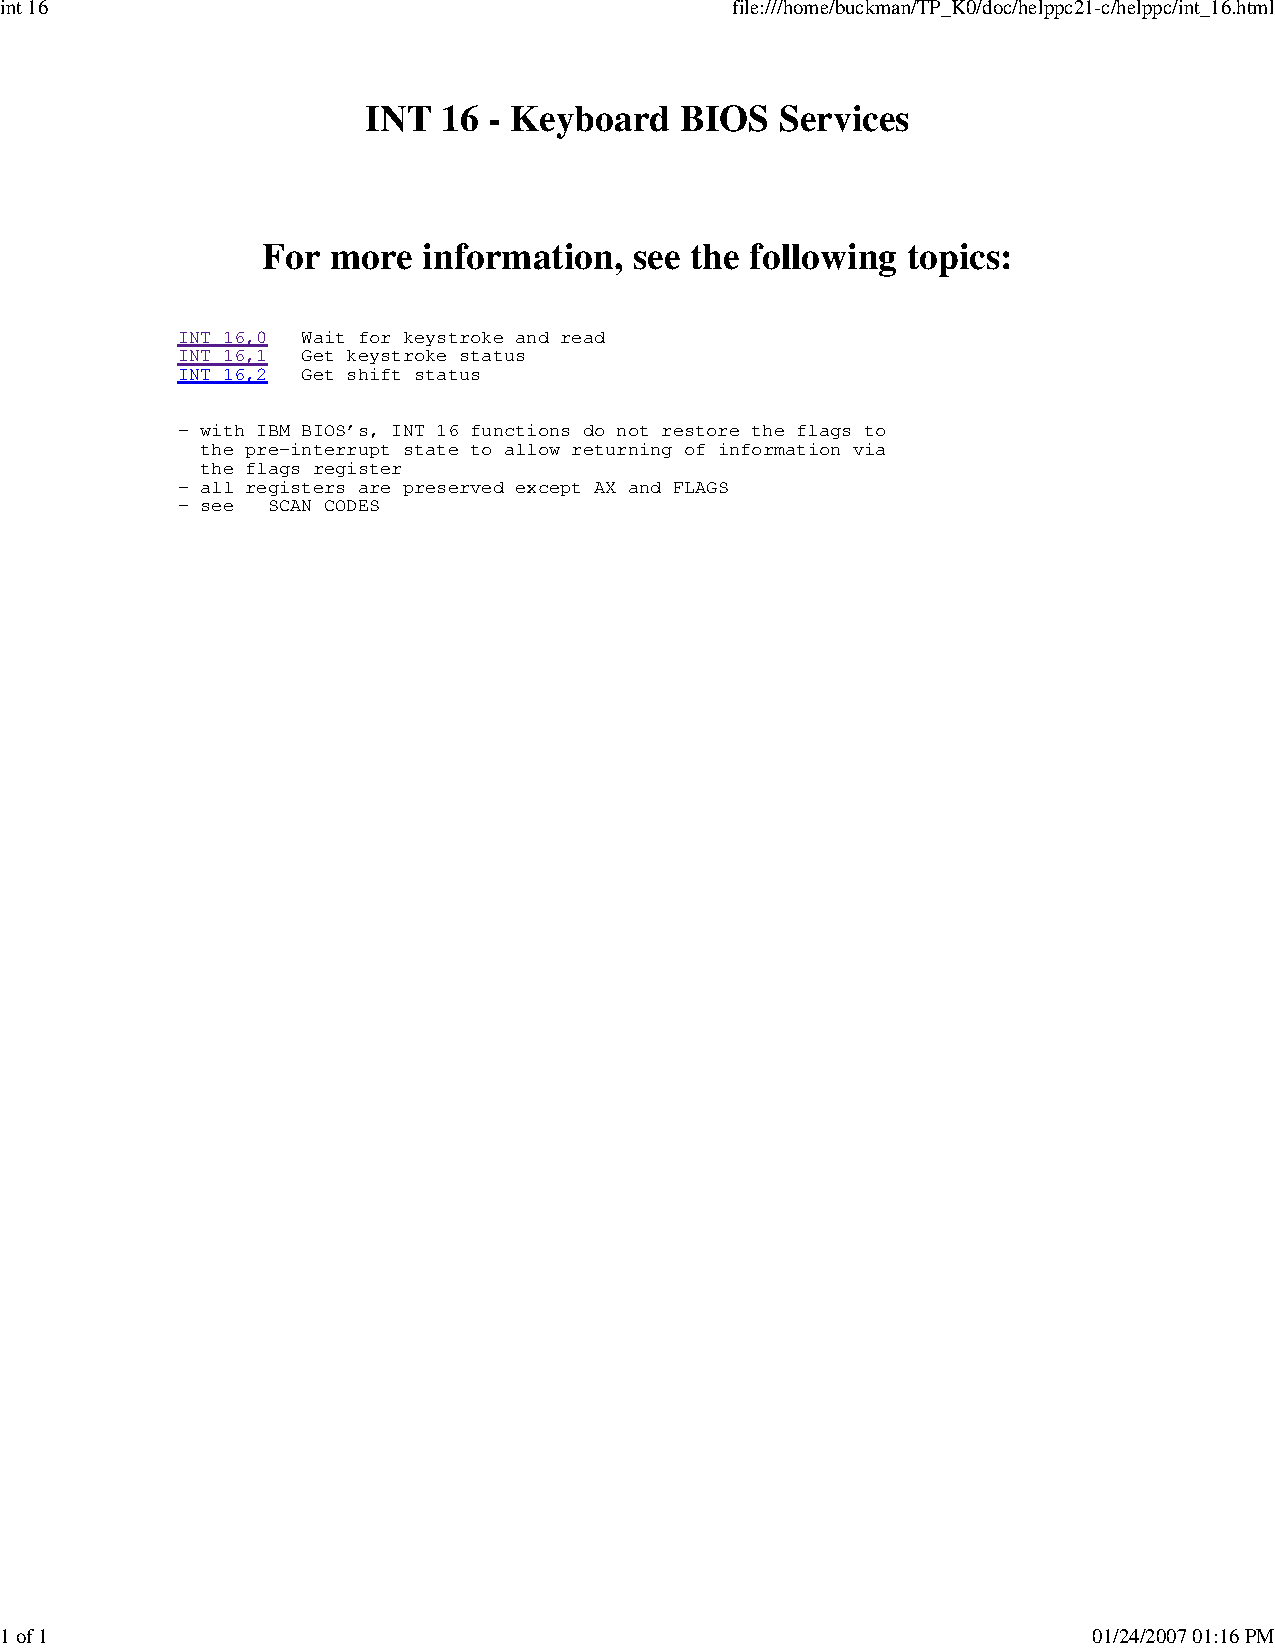
\includepdf[pages=-]{int16}
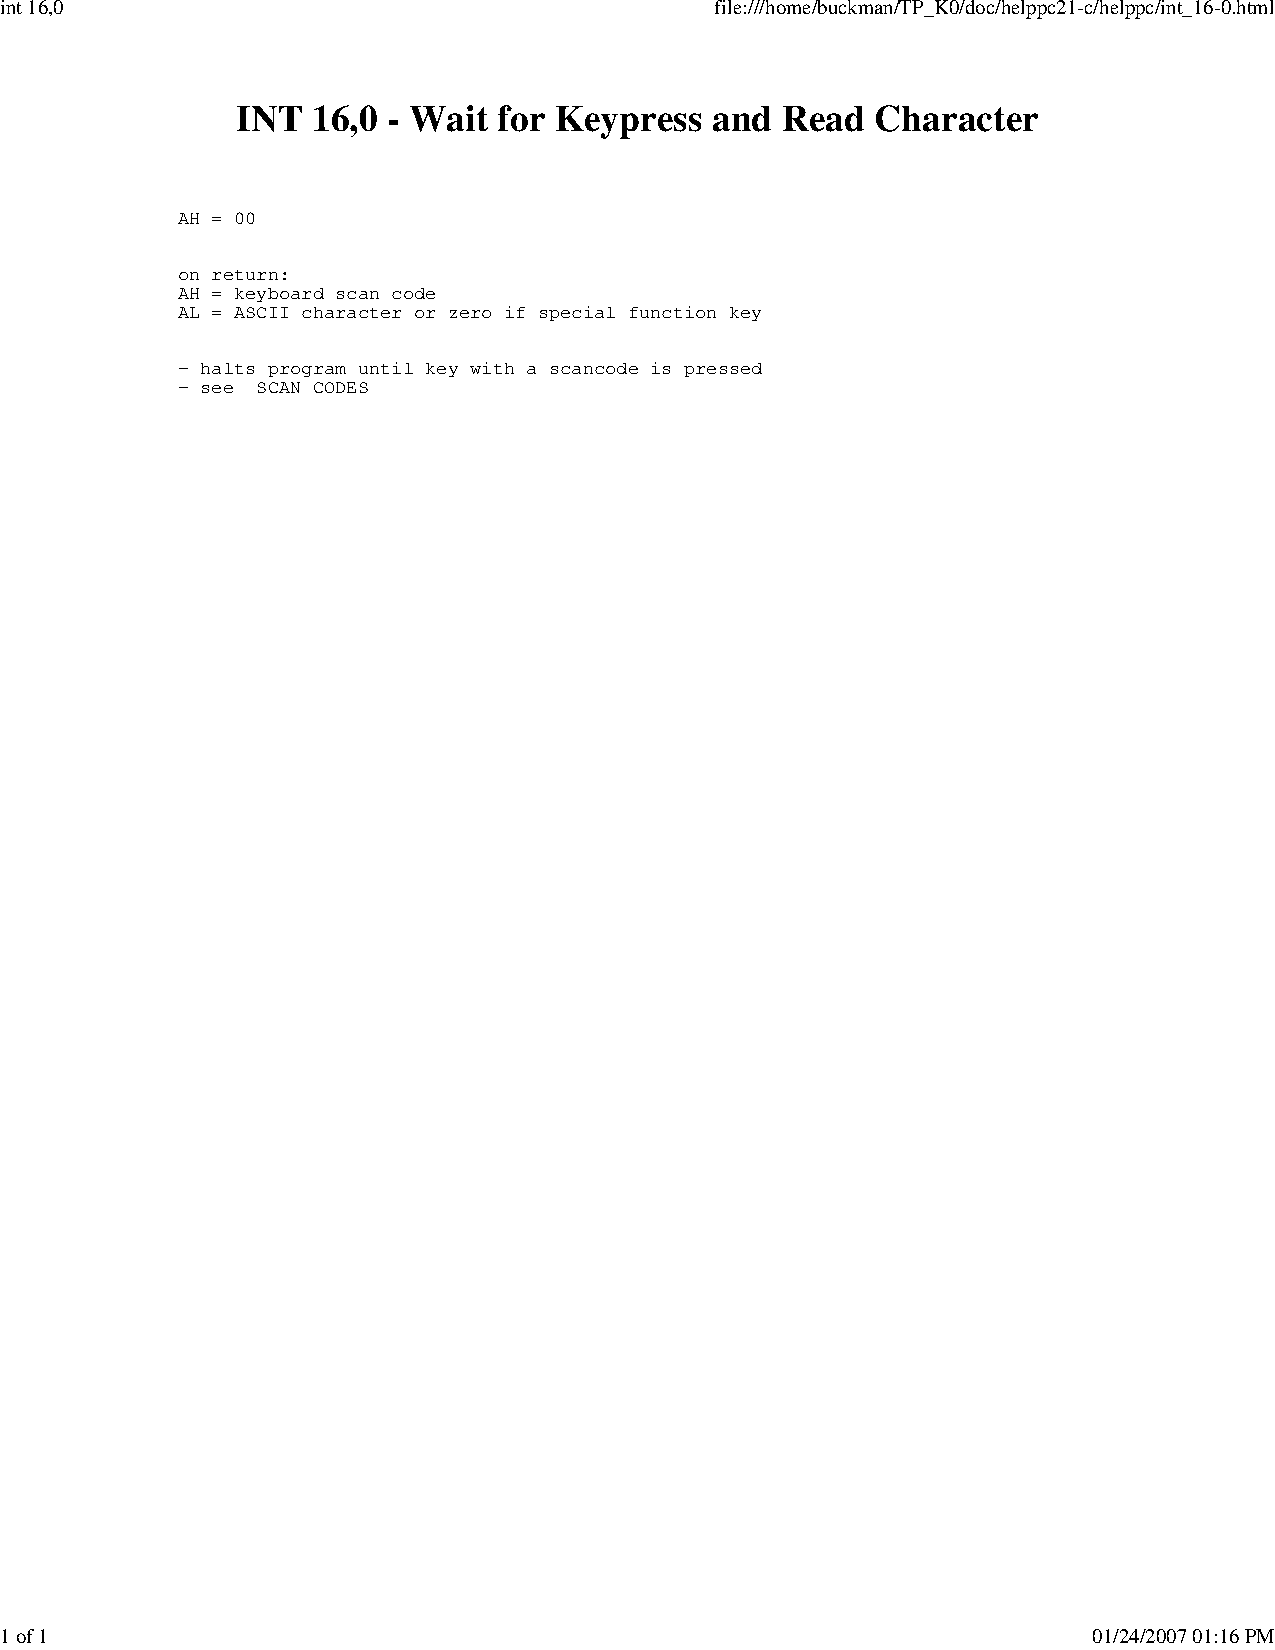
\includepdf[pages=-]{int16_0}
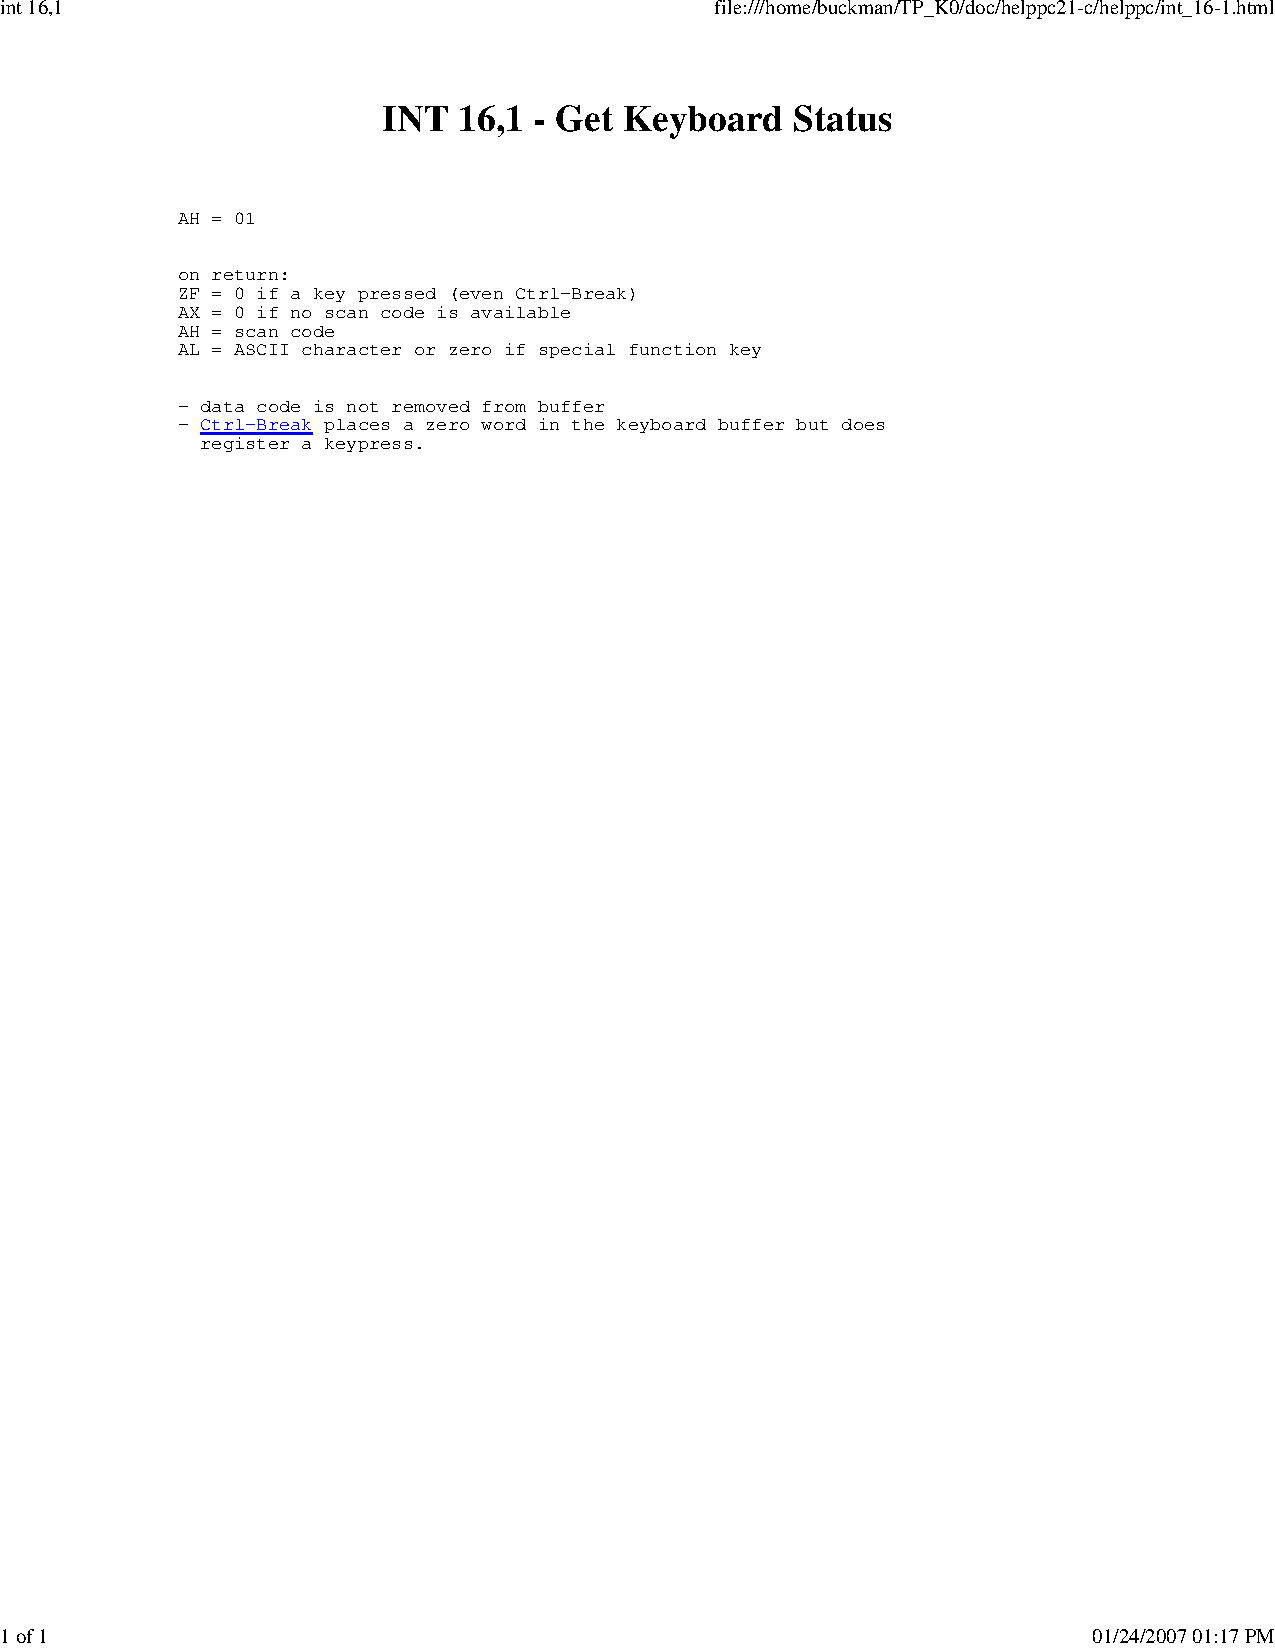
\includepdf[pages=-]{int16_1}
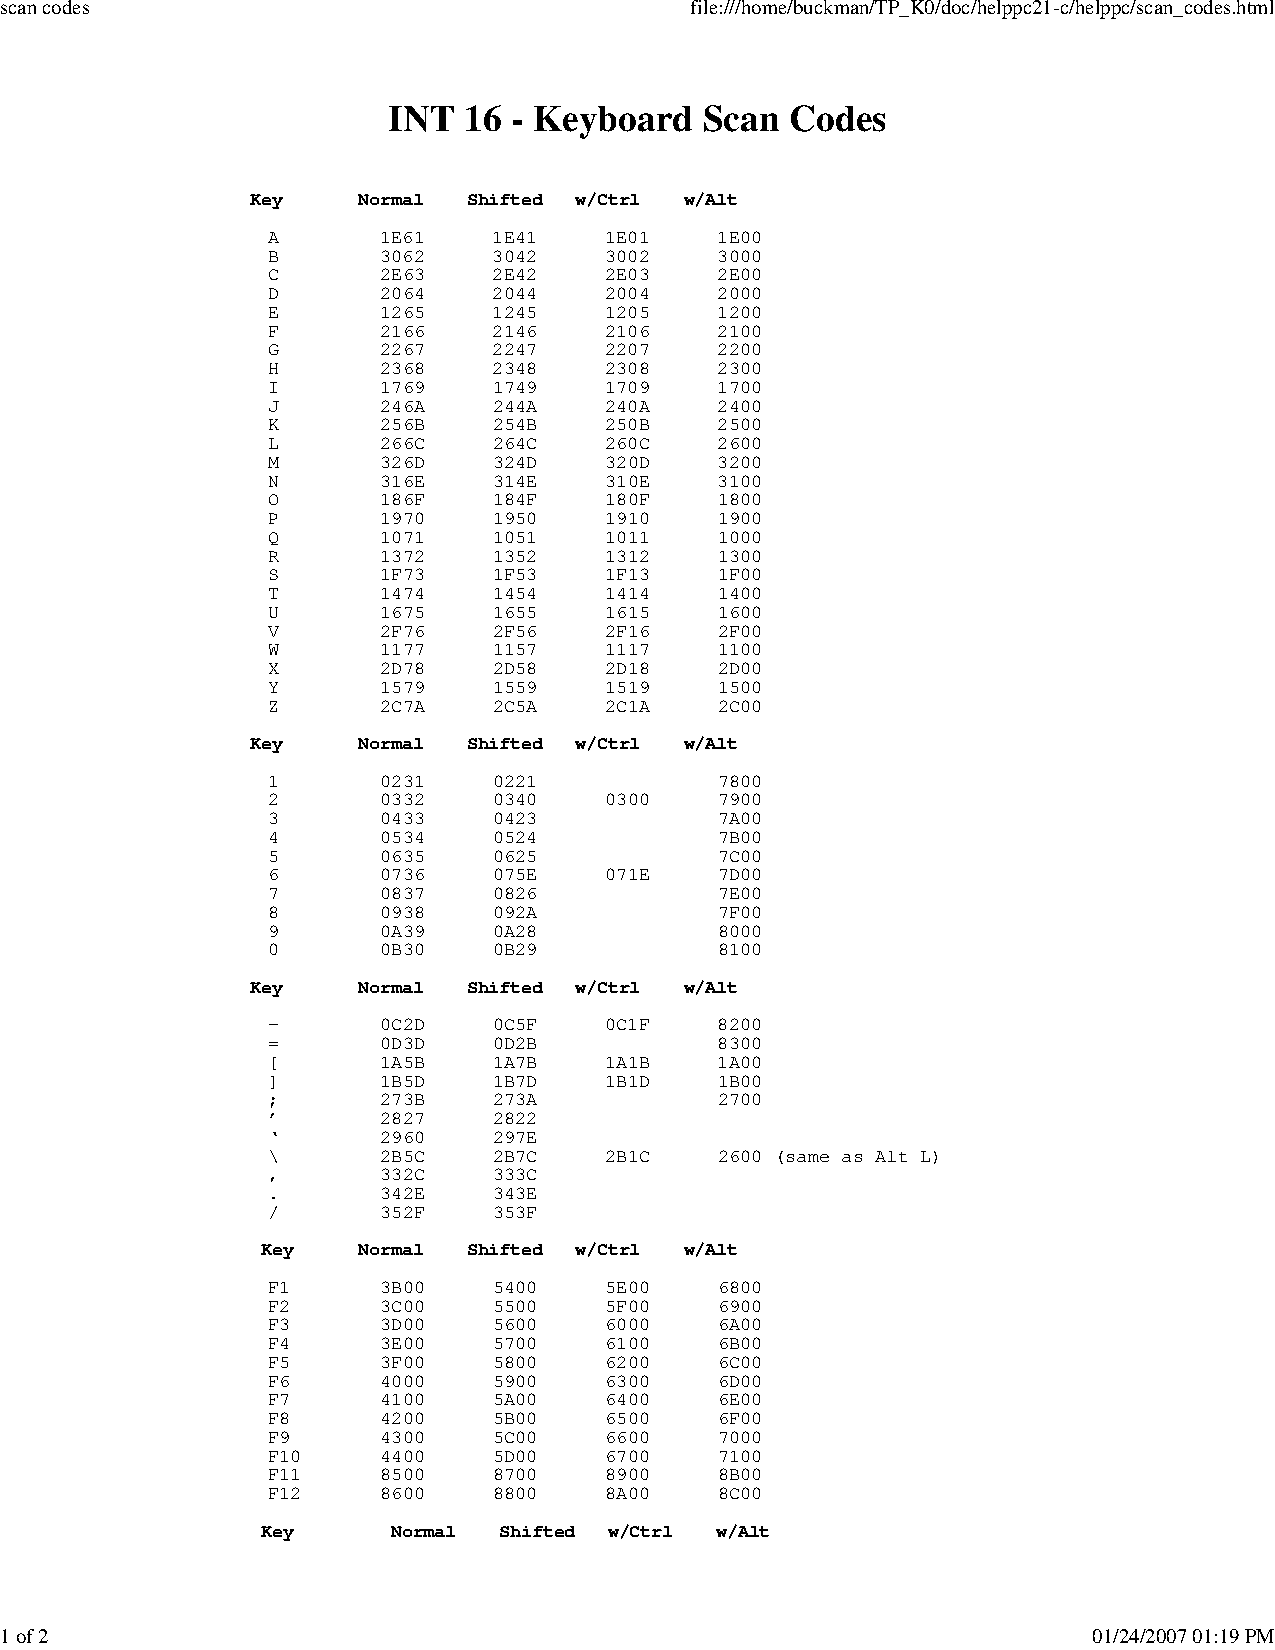
\includepdf[pages=-]{int16_scancodes}

%
% VGA framebuffer
%

\subsection*{VGA Text Framebuffer}

At startup, a VGA card is initialized in color-text mode, with the 80x25
resolution. Each cell is represented by the following couple of bytes:

\begin{center}
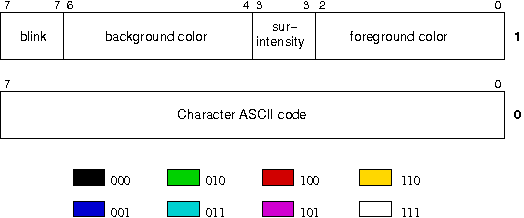
\includegraphics[width=\linewidth]{vga-text}
\end{center}

Write 0x4b at the address 0xb8000 and 0x96 at 0xb8001 will print the
character 'K' blinking in yellow on a blue background, at the top-left corner
of the screen.

%
% ELF documentation
%

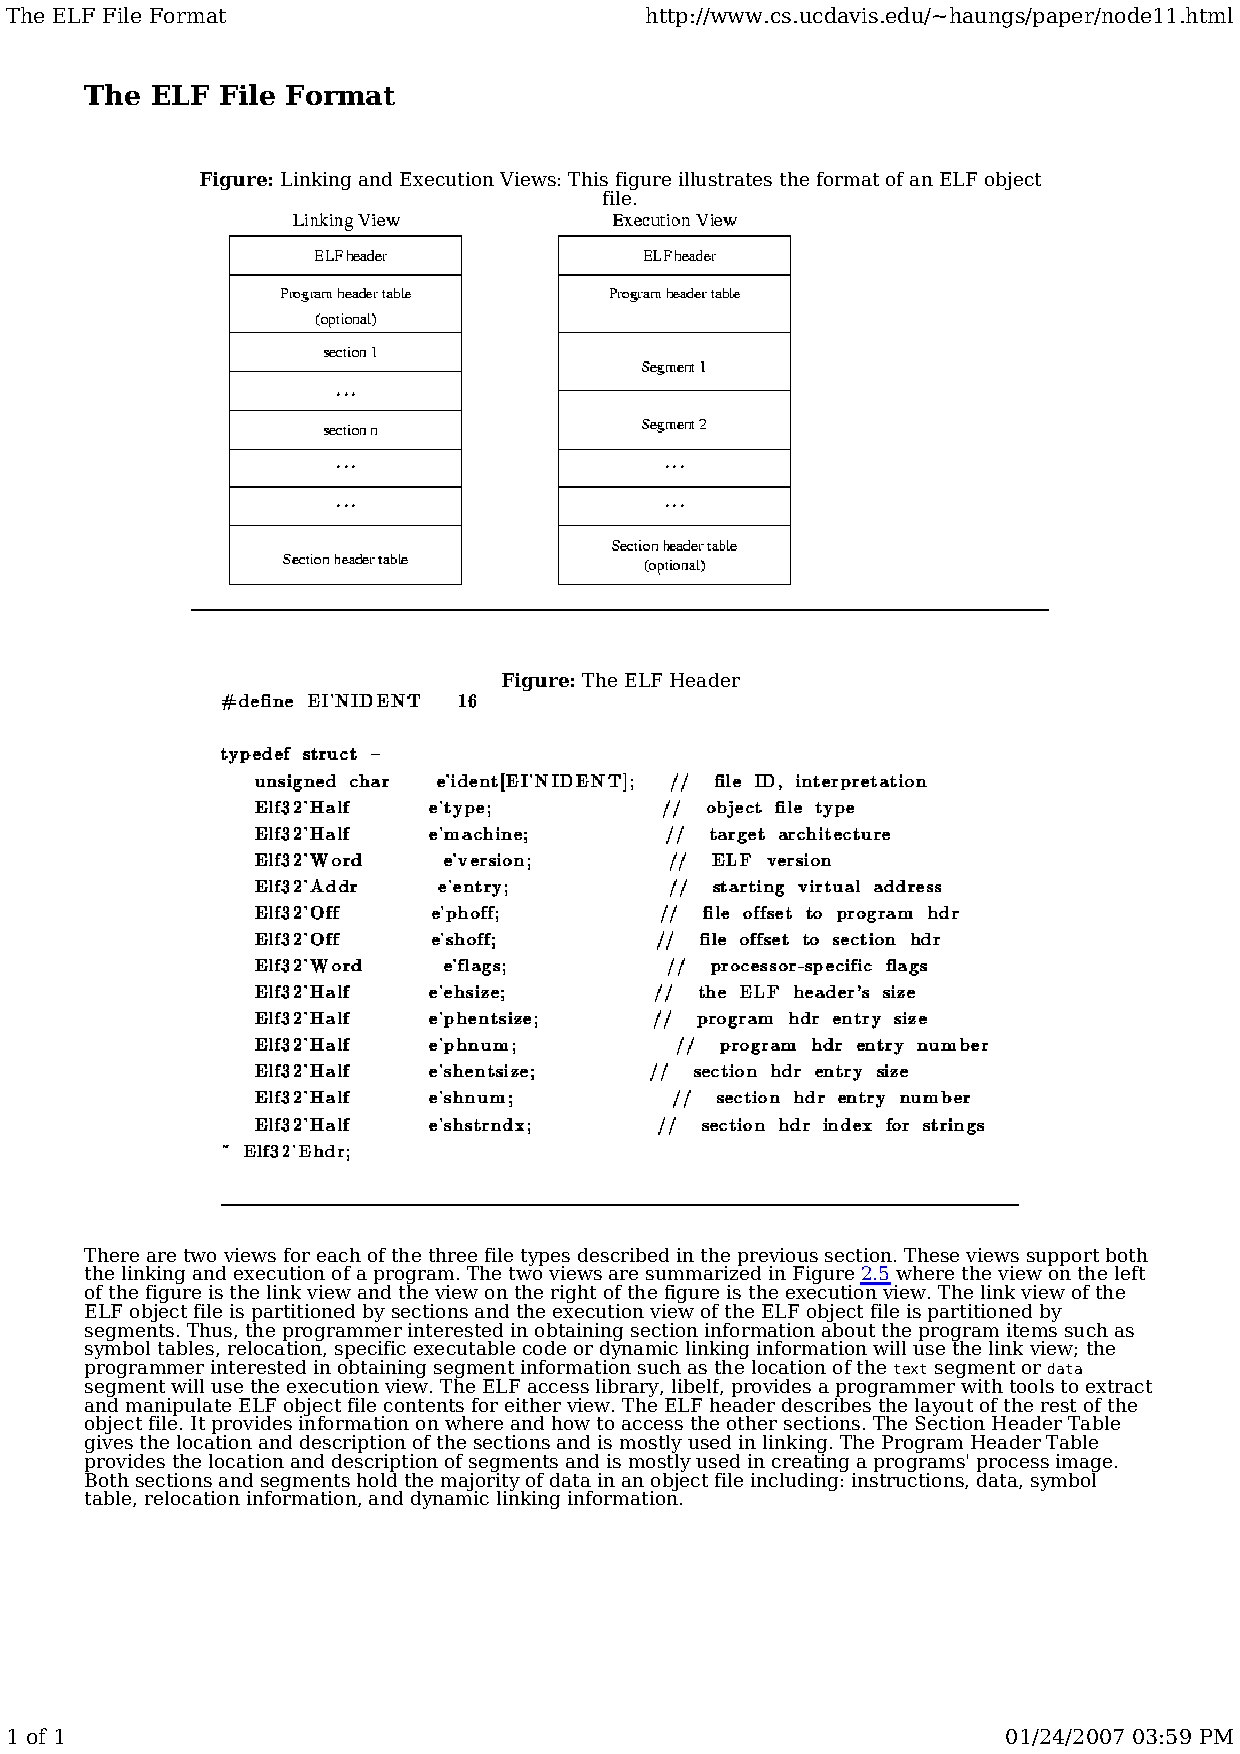
\includepdf[pages=-]{elf1}
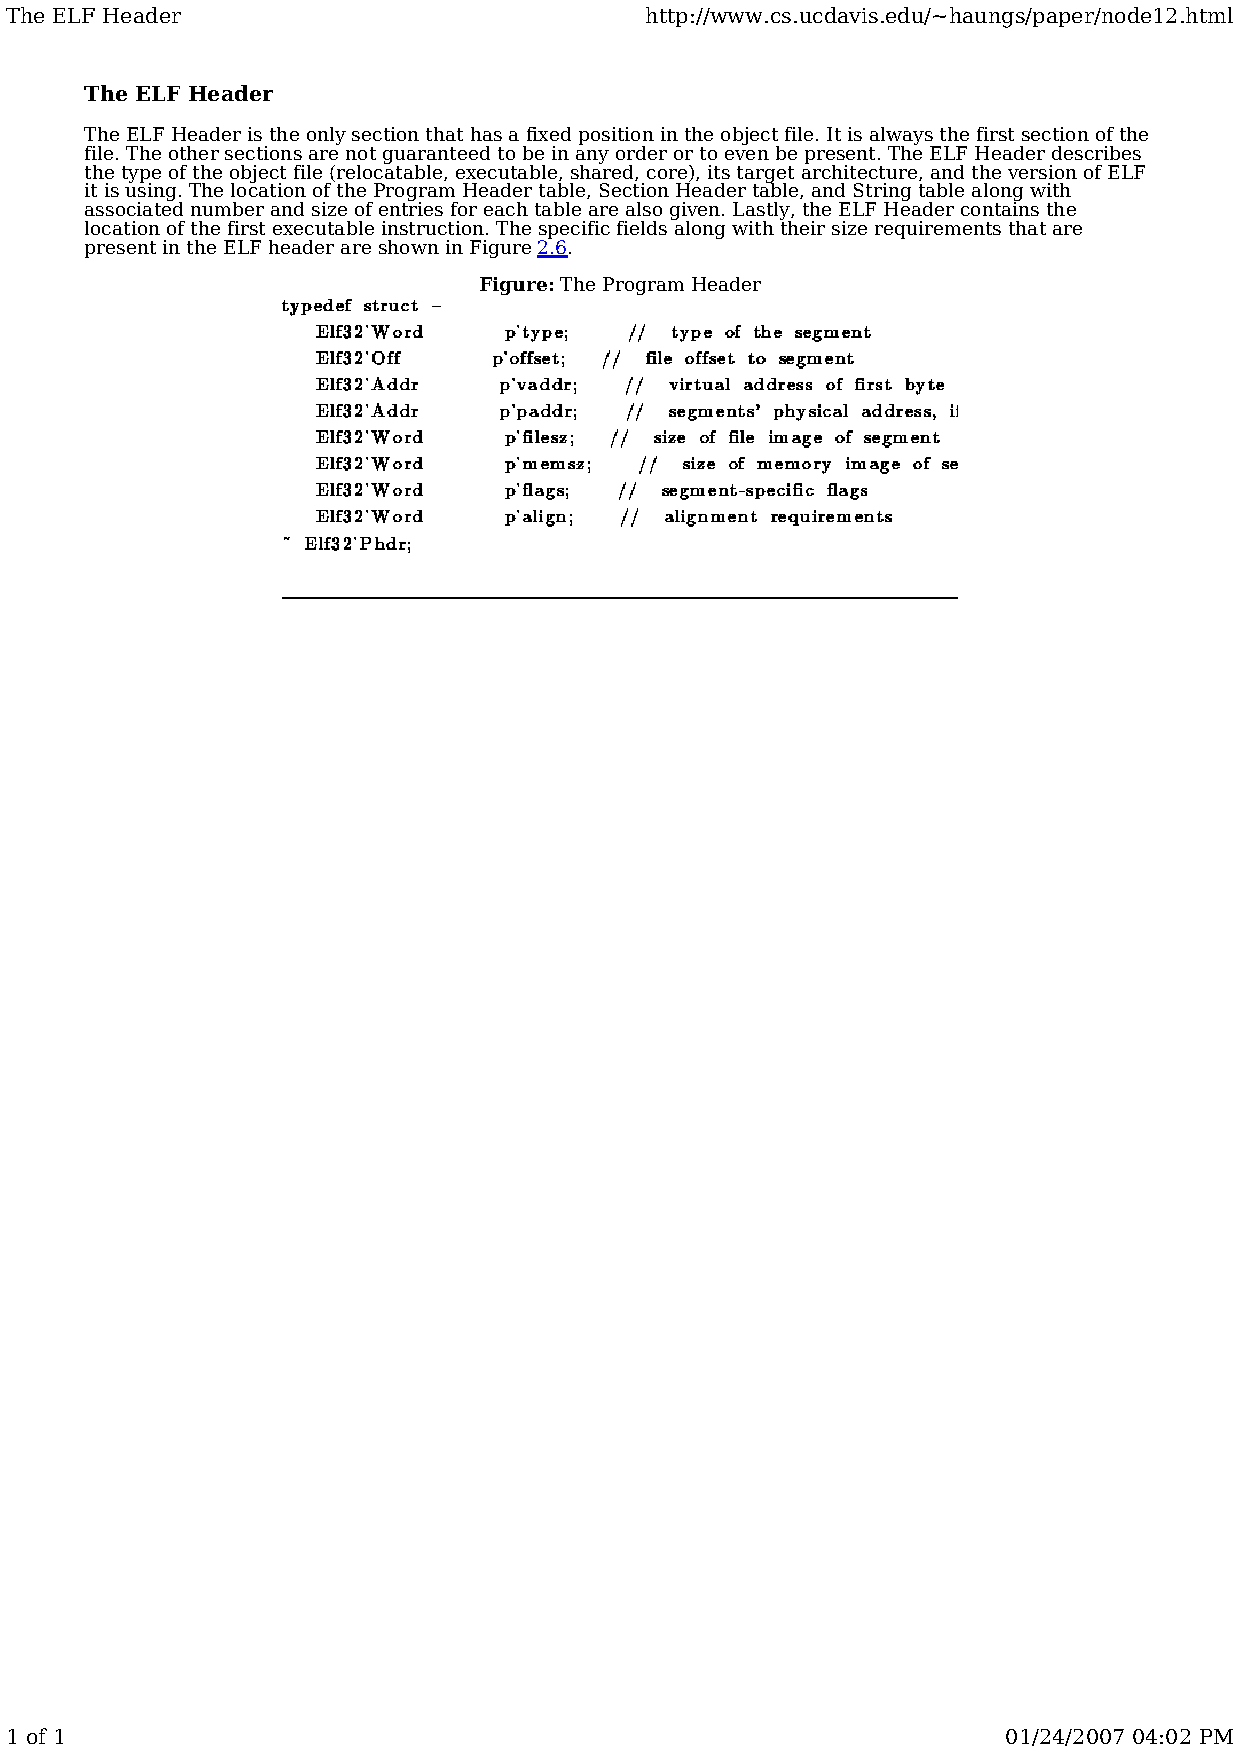
\includepdf[pages=-]{elf2}
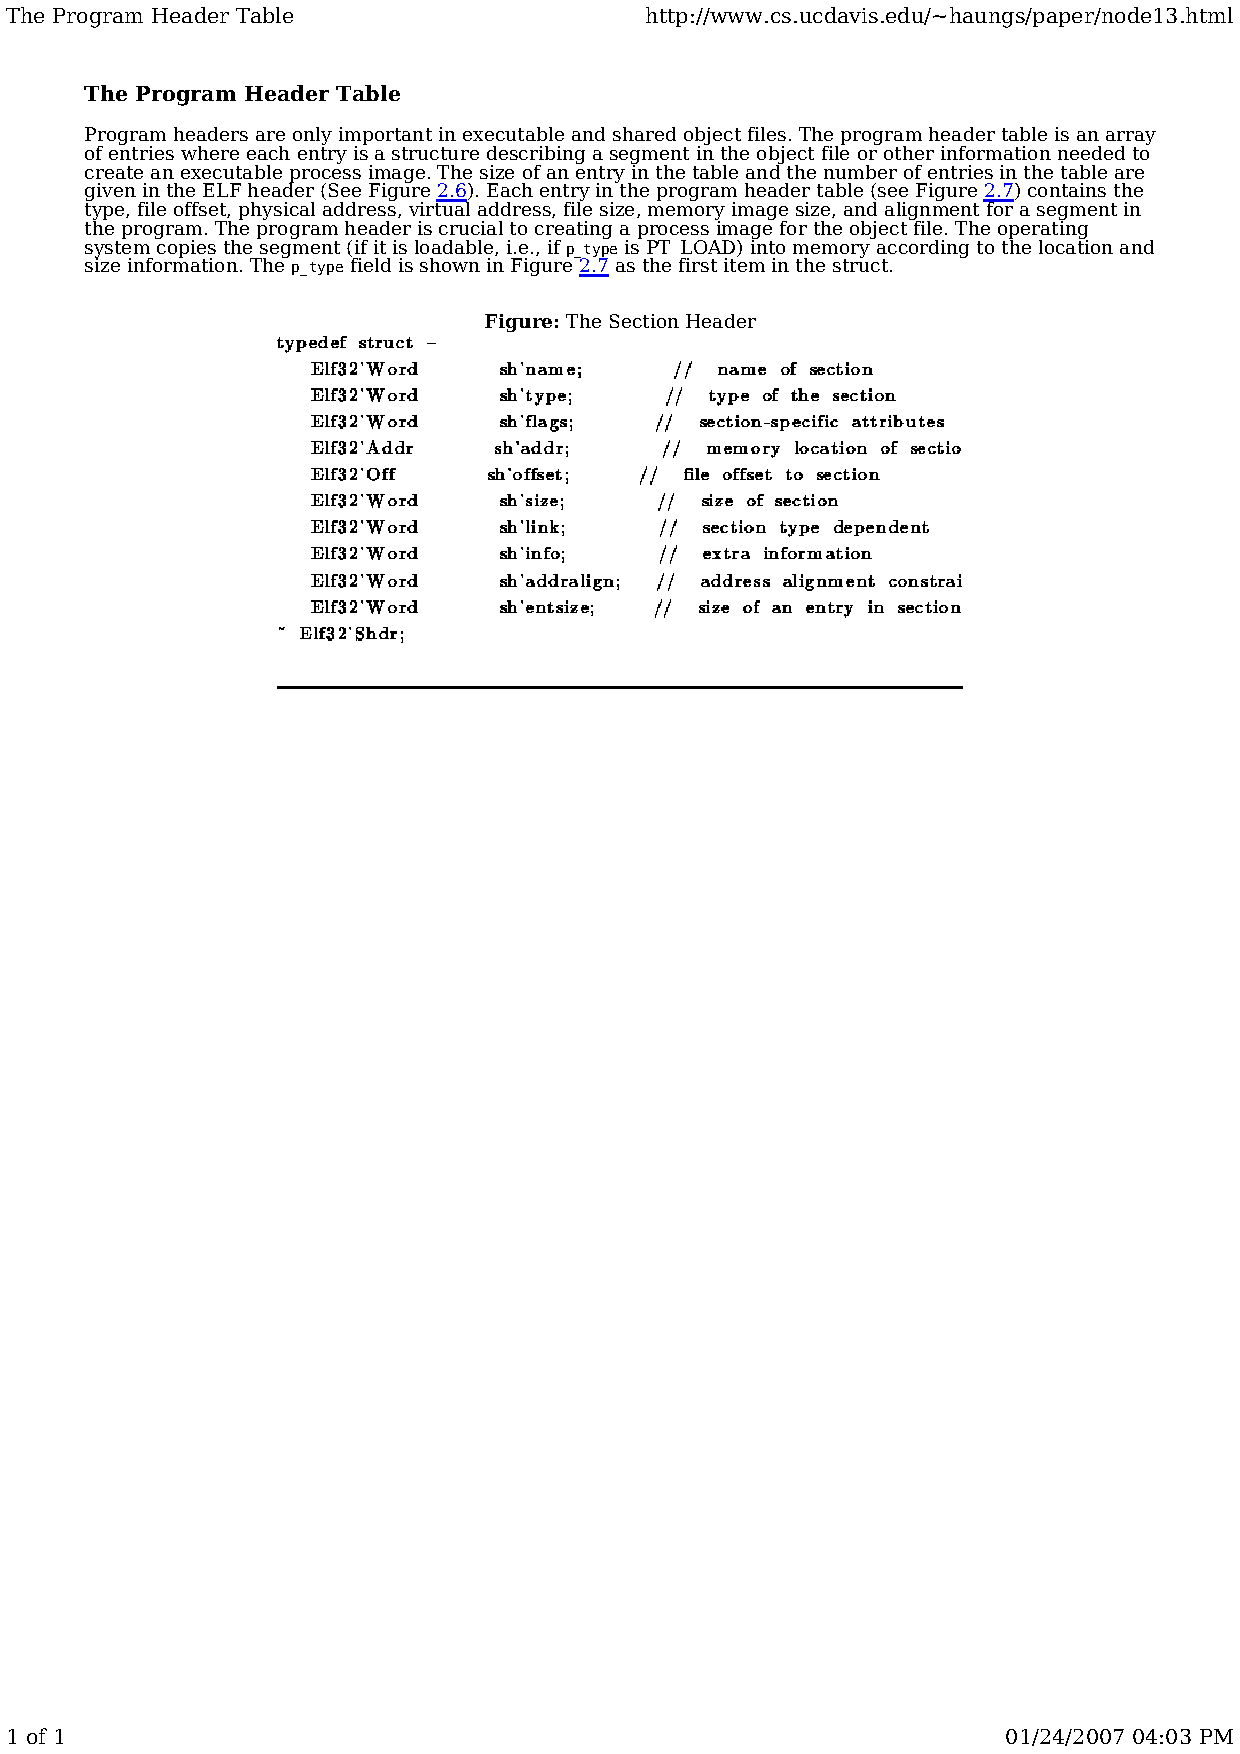
\includepdf[pages=-]{elf3}
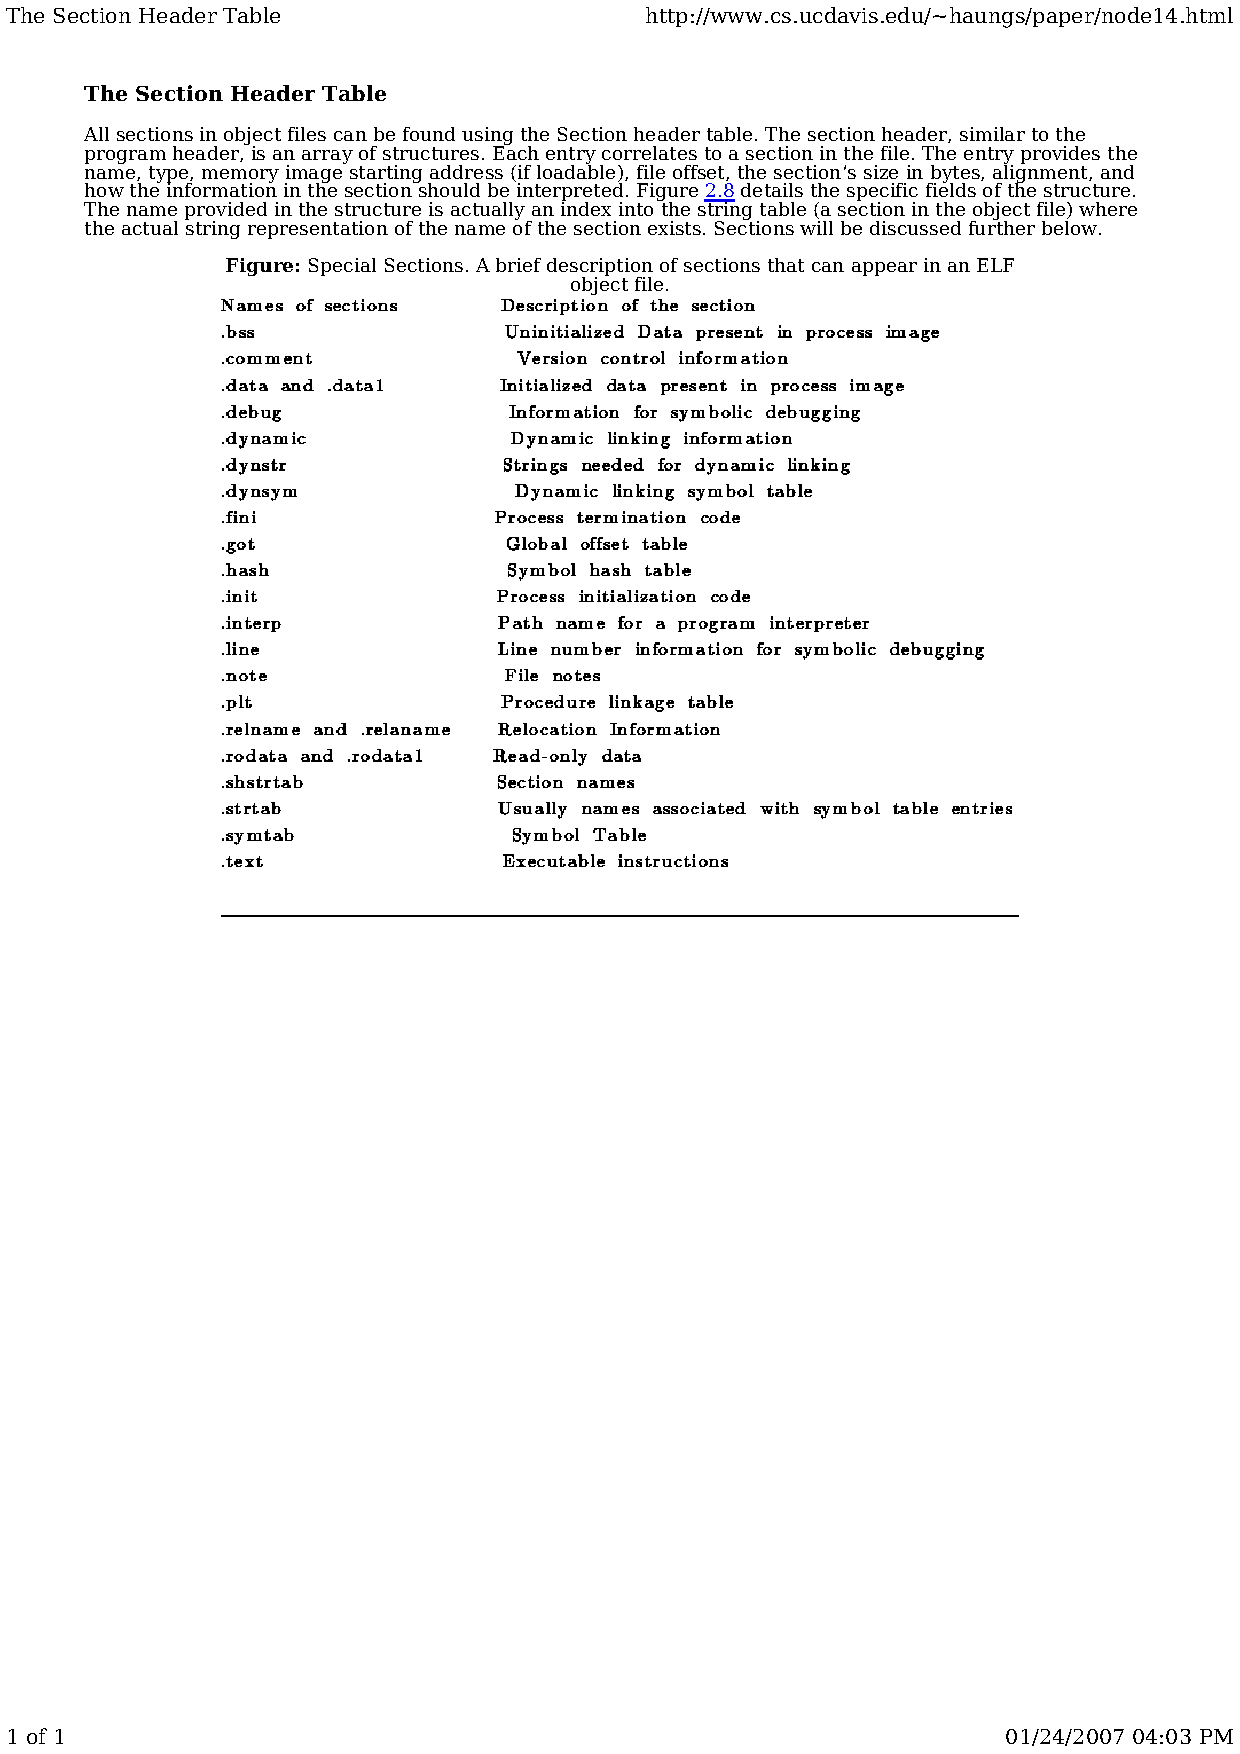
\includepdf[pages=-]{elf4}
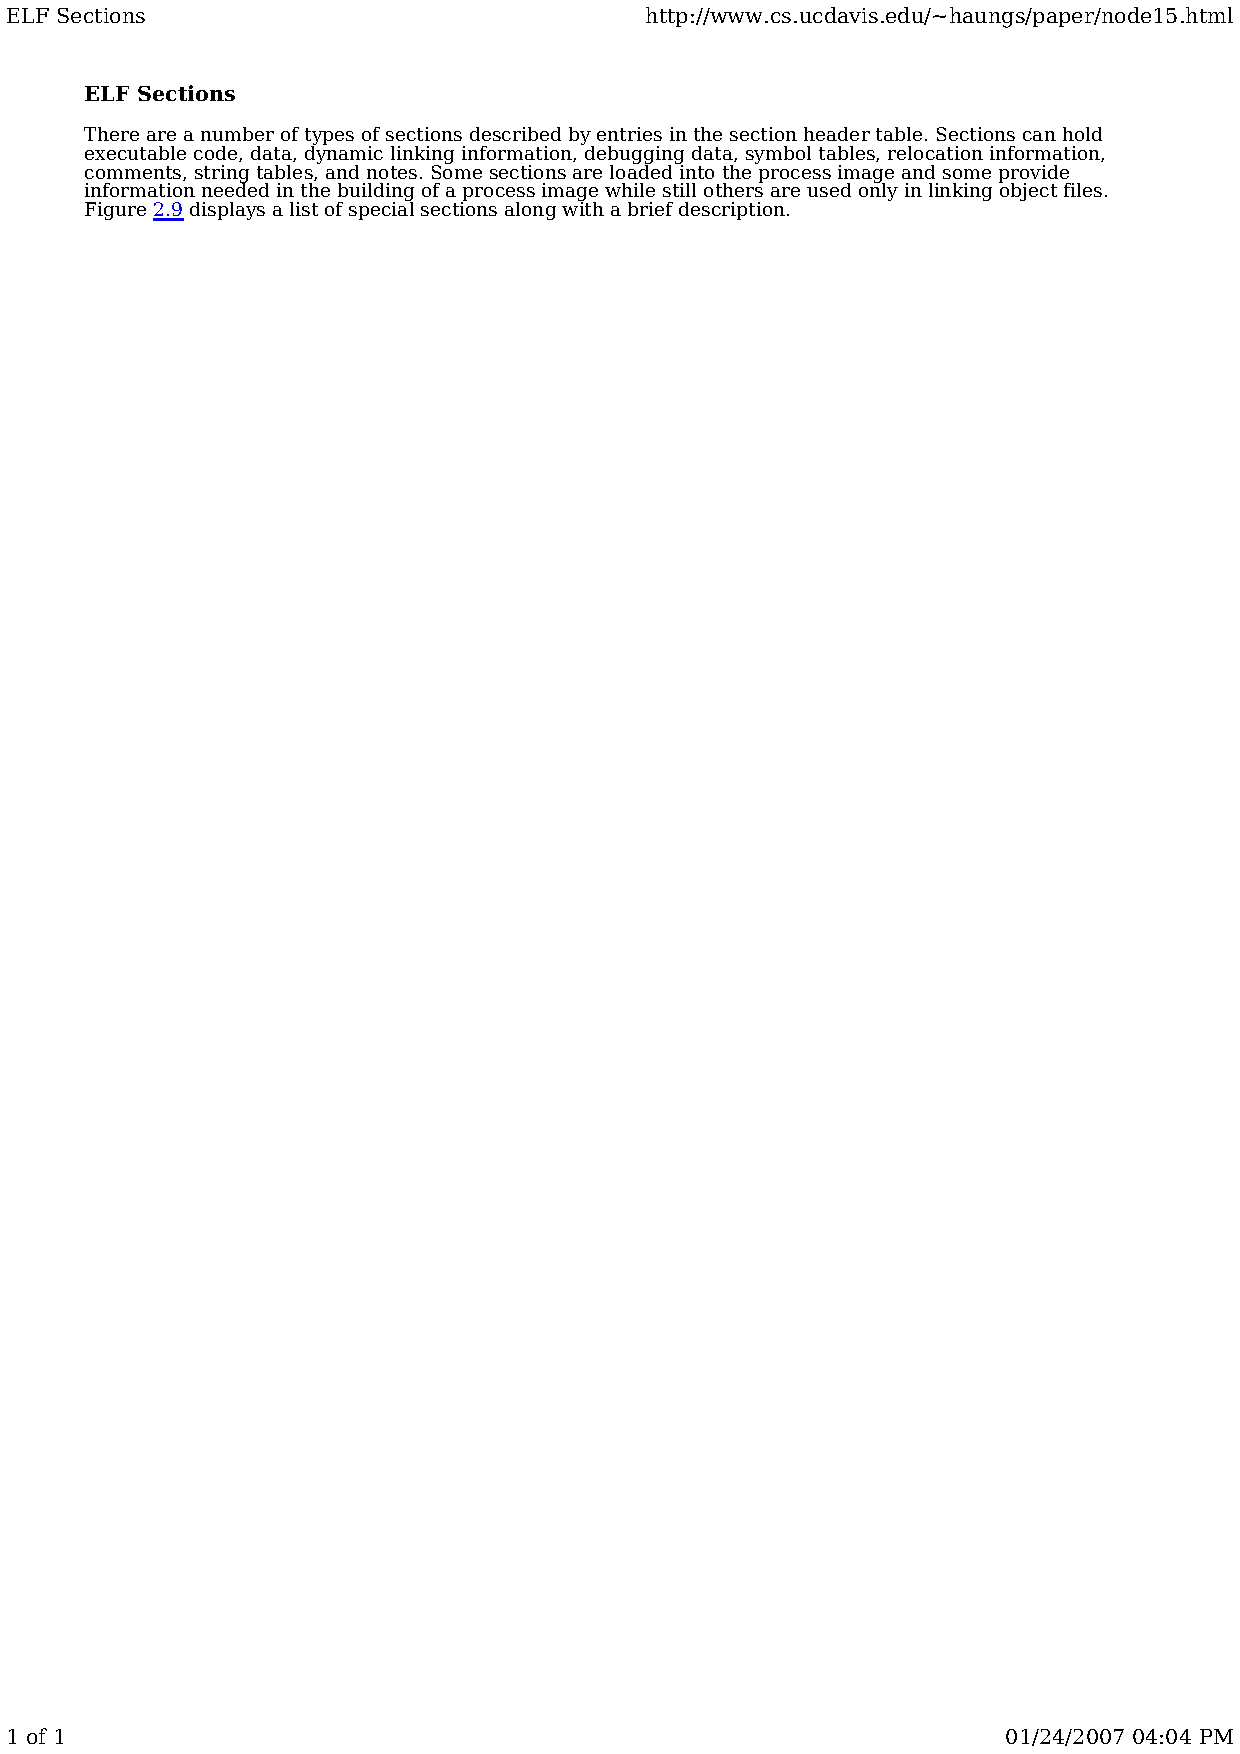
\includepdf[pages=-]{elf5}
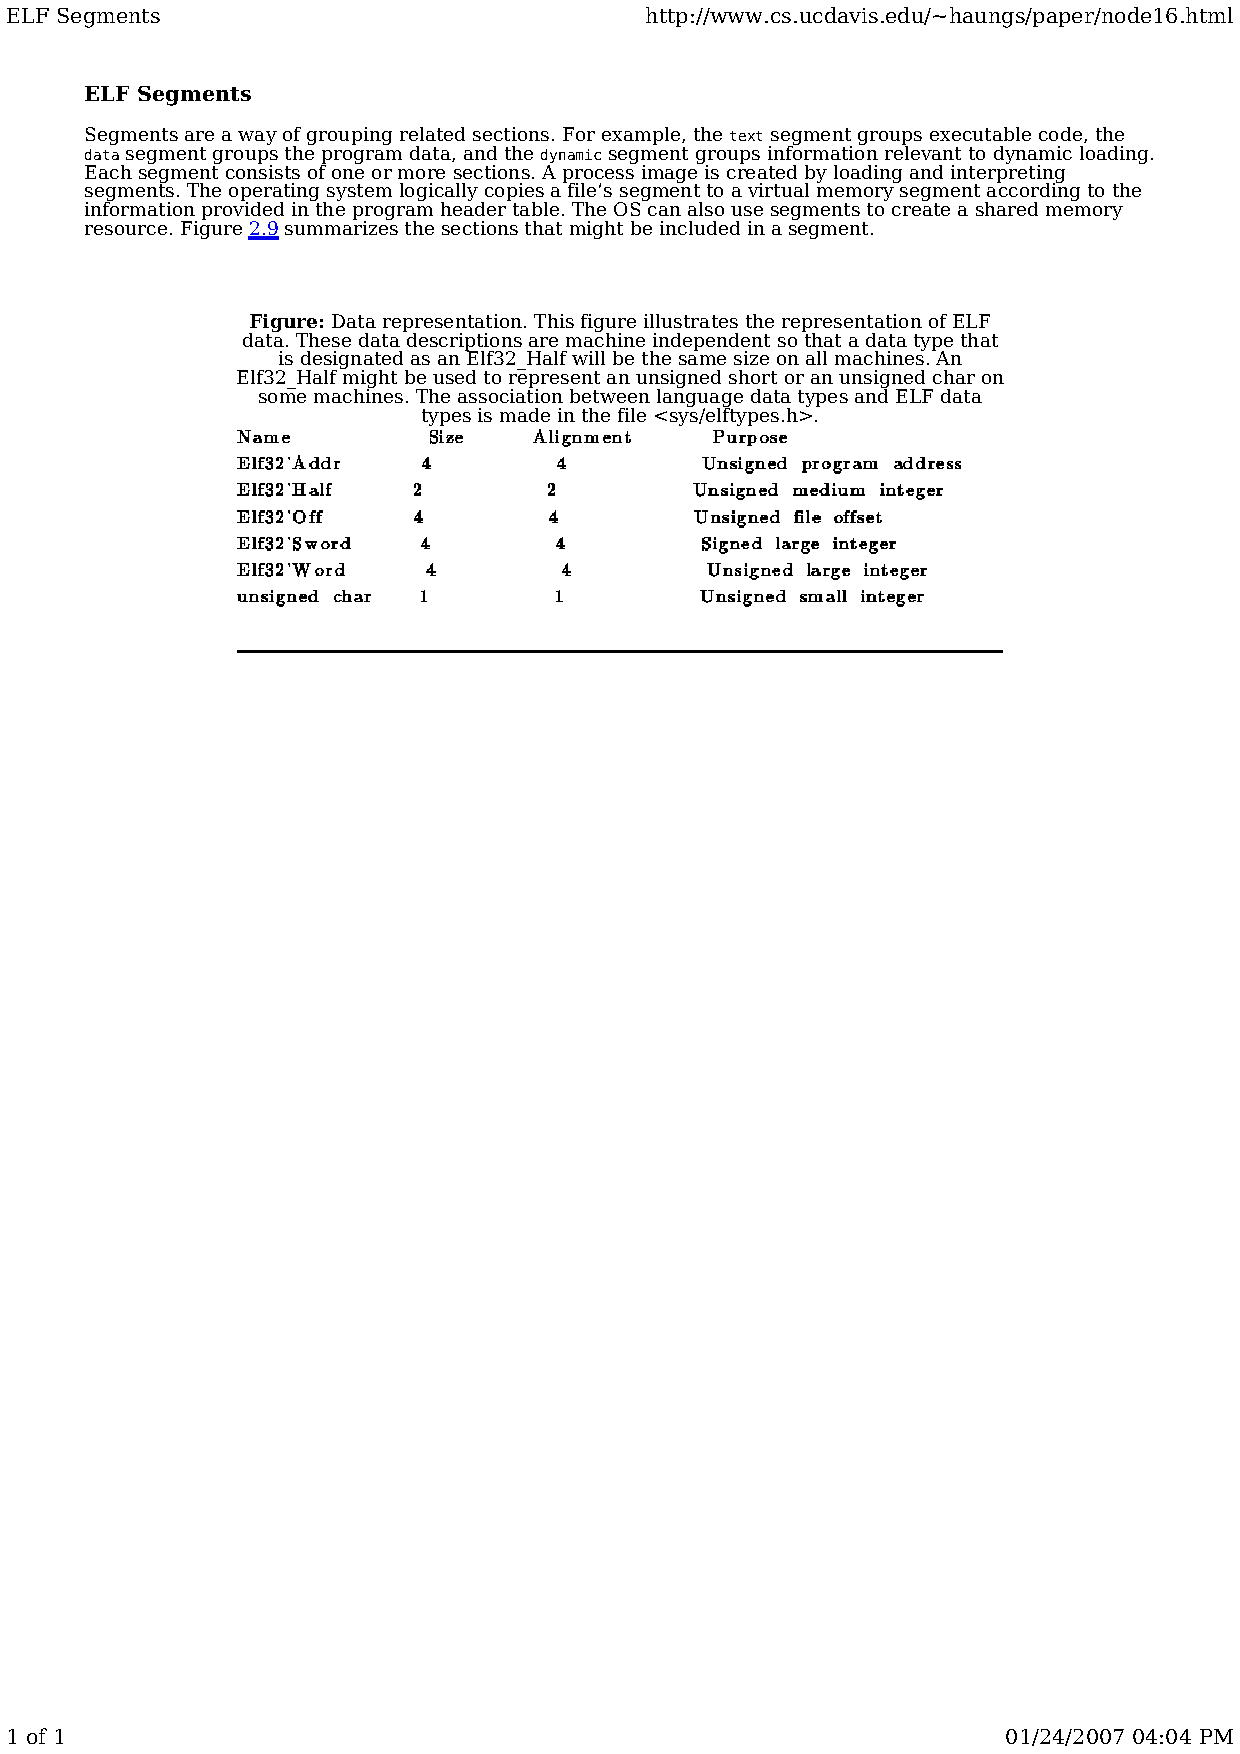
\includepdf[pages=-]{elf6}
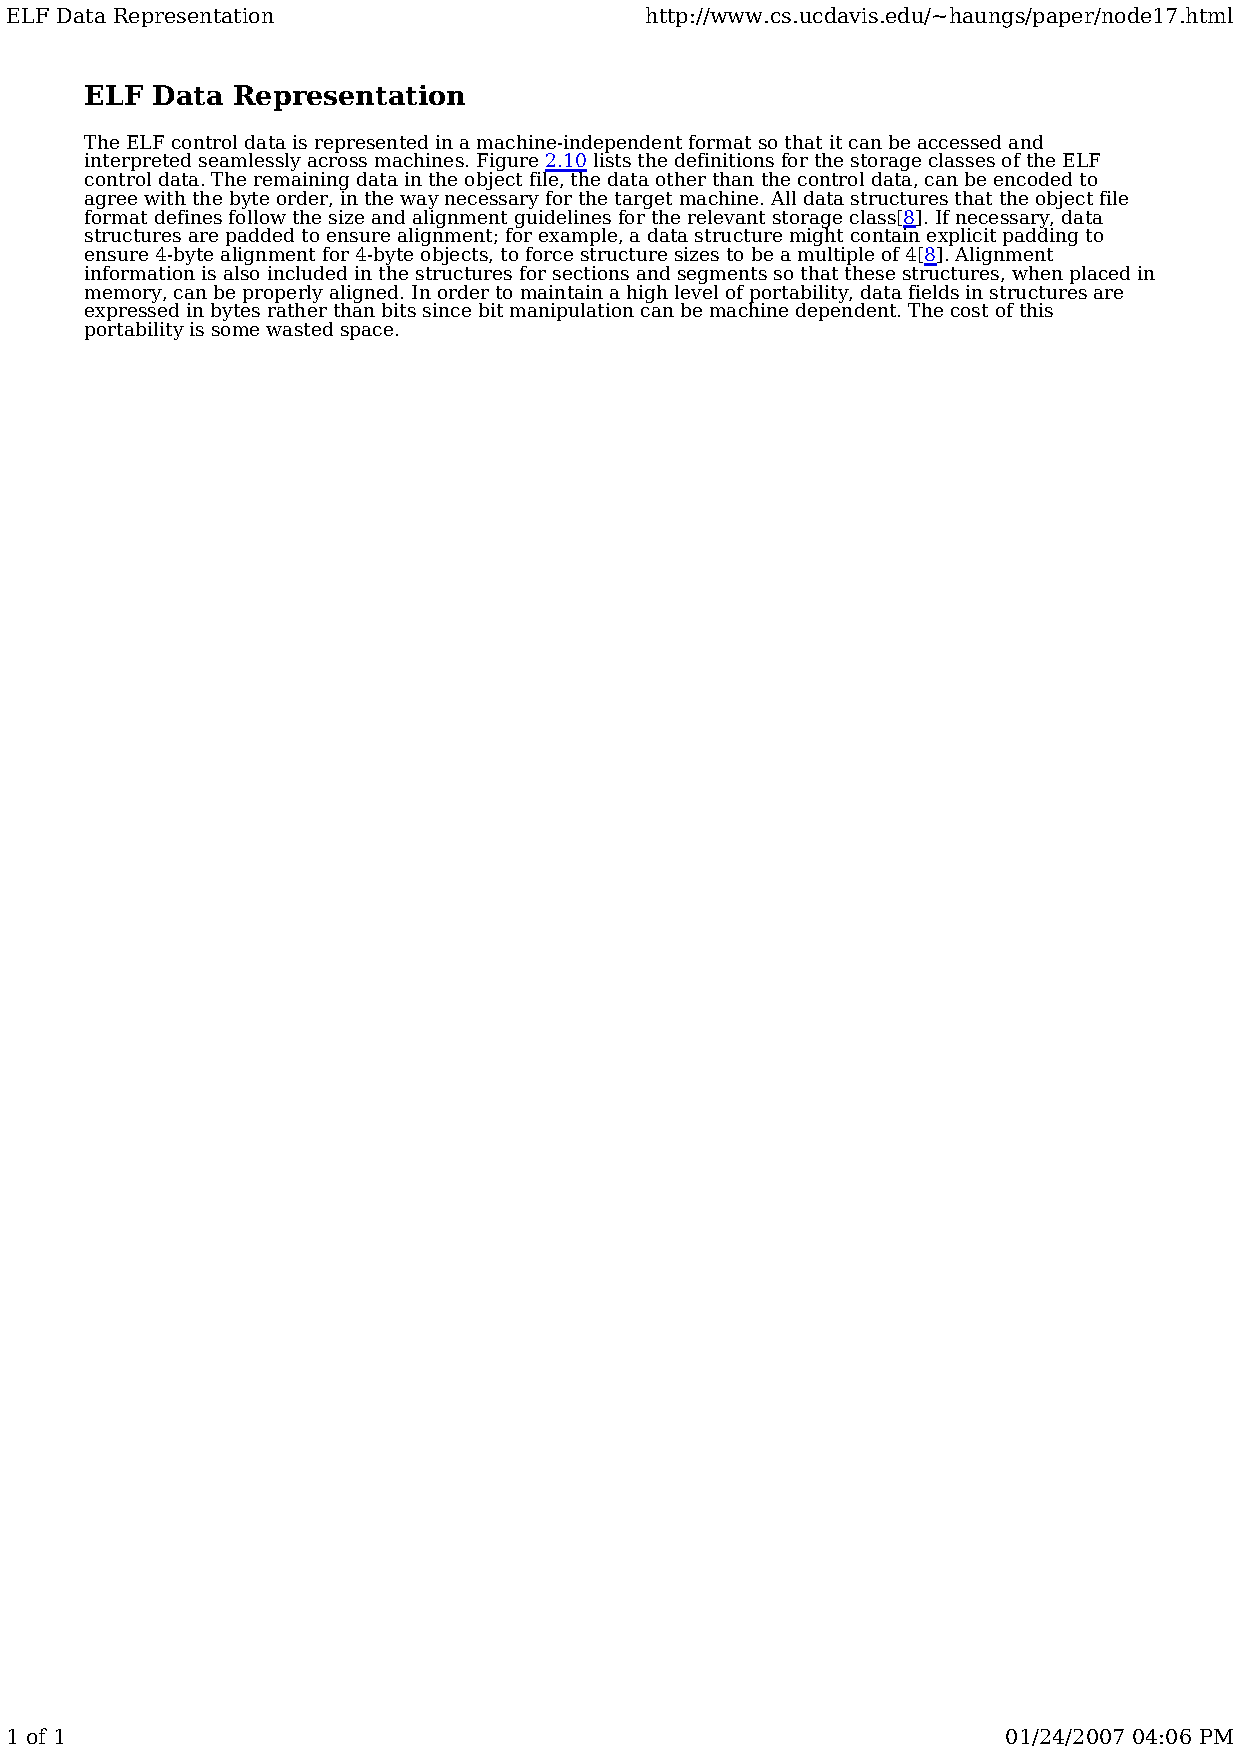
\includepdf[pages=-]{elf7}

%
% IA-32 operating mode switch
%

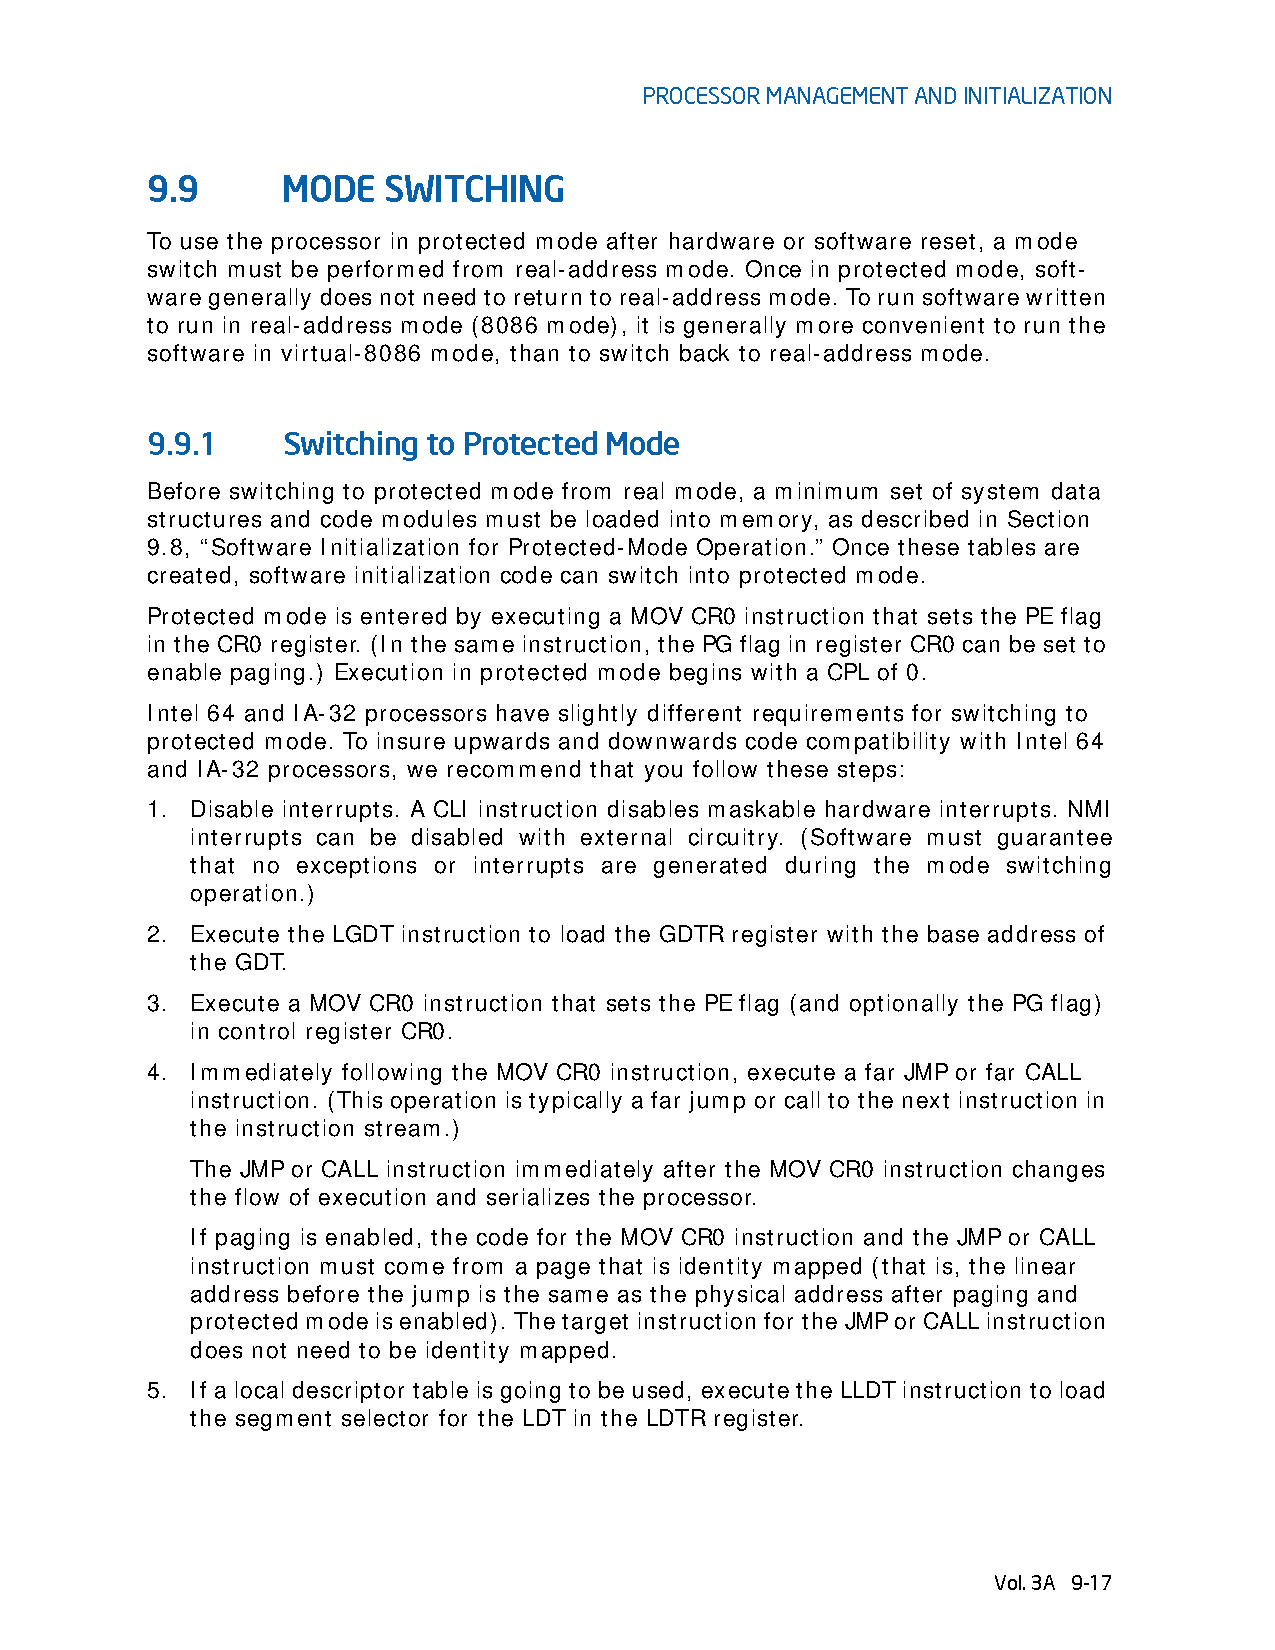
\includepdf[pages=-]{mode_switch}

\end{document}
